\documentclass[a4paper,12pt]{report}

\usepackage[utf8]{inputenc}
\usepackage{amsmath}
\usepackage{fontspec}
\usepackage{float}
\usepackage{enumitem}
\usepackage{graphicx}
\usepackage{wrapfig}
\usepackage{setspace}
\usepackage{mathtools}
\usepackage{textgreek}
\usepackage{gensymb}
\usepackage[titletoc]{appendix}
\usepackage{longtable}
\usepackage{makecell}
\usepackage{pdfpages} 
\usepackage{cite}
\usepackage{url}
\usepackage{listings}
\usepackage{color}
\usepackage{subcaption}
\usepackage[redeflists]{IEEEtrantools}

\definecolor{codegreen}{rgb}{0,0.6,0}
\definecolor{codegray}{rgb}{0.5,0.5,0.5}
\definecolor{codepurple}{rgb}{0.58,0,0.82}

\lstdefinestyle{mystyle}{
	backgroundcolor=\color{white},   
	commentstyle=\color{codegreen},
	keywordstyle=\color{blue},
	numberstyle=\tiny\color{codegray},
	stringstyle=\color{codepurple},
	basicstyle=\footnotesize,
	breakatwhitespace=false,         
	breaklines=true,                 
	captionpos=b,                    
	keepspaces=true,                 
	numbers=left,                    
	numbersep=5pt,                  
	showspaces=false,                
	showstringspaces=false,
	showtabs=false,                  
	tabsize=2
}

\lstset{style=mystyle}

\setlength{\parindent}{0em}
\setlength{\parskip}{0.5em}

\setmainfont[
BoldFont=arialbd.ttf,
ItalicFont=ariali.ttf,
BoldItalicFont=arialbi.ttf
]{arial.ttf}

\author{Arundathi Shaji Shanthini}


\renewcommand{\bibname}{References}

\begin{document}
\bstctlcite{IEEEexample:BSTcontrol}
%%%%%%%%%%%COVERSHEET%%%%%%%%%%%%%%%%%
\begin{titlepage}
    %\setlength{\voffset}{-1.8in}
    \noindent \noindent
	\begin{figure}[t]
		\vspace{-1.8in}
		\hspace{-1.5in}
		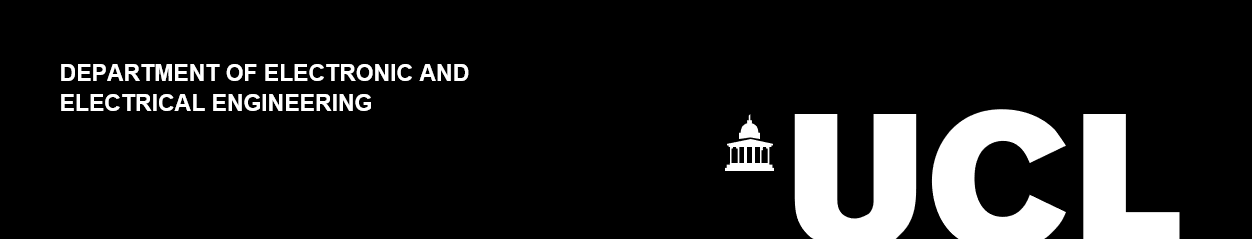
\includegraphics[width=1.55\textwidth]{images/Coversheet_Header_black_with_text.png}
	\end{figure}
   
    \vspace{15mm}

    \begin{center}
        {\LARGE \textbf{BEng Project}}\\
        \vspace{4mm}
        {\Huge \textbf{Final Report}}
    \end{center}
    
    \vspace{10mm}
    
    \begin{center}
    \begin{spacing}{1.8}
    {\LARGE
   Dynamic Modelling of a Continuum Robotic Snake-arm and its Performance Evaluation by Analysing Robustness}
    \end{spacing}
    
    
   \vspace{25mm}
    
    \begingroup
    \renewcommand{\arraystretch}{1.3}
    
     \begin{tabular}[!b]{ll}
        \textbf{Student Name:}  & \hspace{4mm} Arundathi Shaji Shanthini \\
       \textbf{Contact e-mail:} & \hspace{4mm} arundathi.shanthini.16@ucl.ac.uk \\
        \textbf{Student number:} & \hspace{4mm} 16018351 \\ \\ 
        \textbf{Project Supervisor:}  & \hspace{4mm} Prof. Sarah Spurgeon \\
        \textbf{Contact e-mail:}  & \hspace{4mm} s.spurgeon@ucl.ac.uk \\
         \textbf{Department:} & \hspace{4mm} \makecell[l]{Department of Electronic and \\Electrical Engineering}\\ \\ 
          \textbf{Submission Date:} & \hspace{4mm} 21\textsuperscript{st} of April 2020      
    \end{tabular}
	\endgroup
\end{center}
\end{titlepage}
%%%%%%%%%%%%%%%%%%%%%%%%%%%%%%%%%%%%%%

\pagebreak

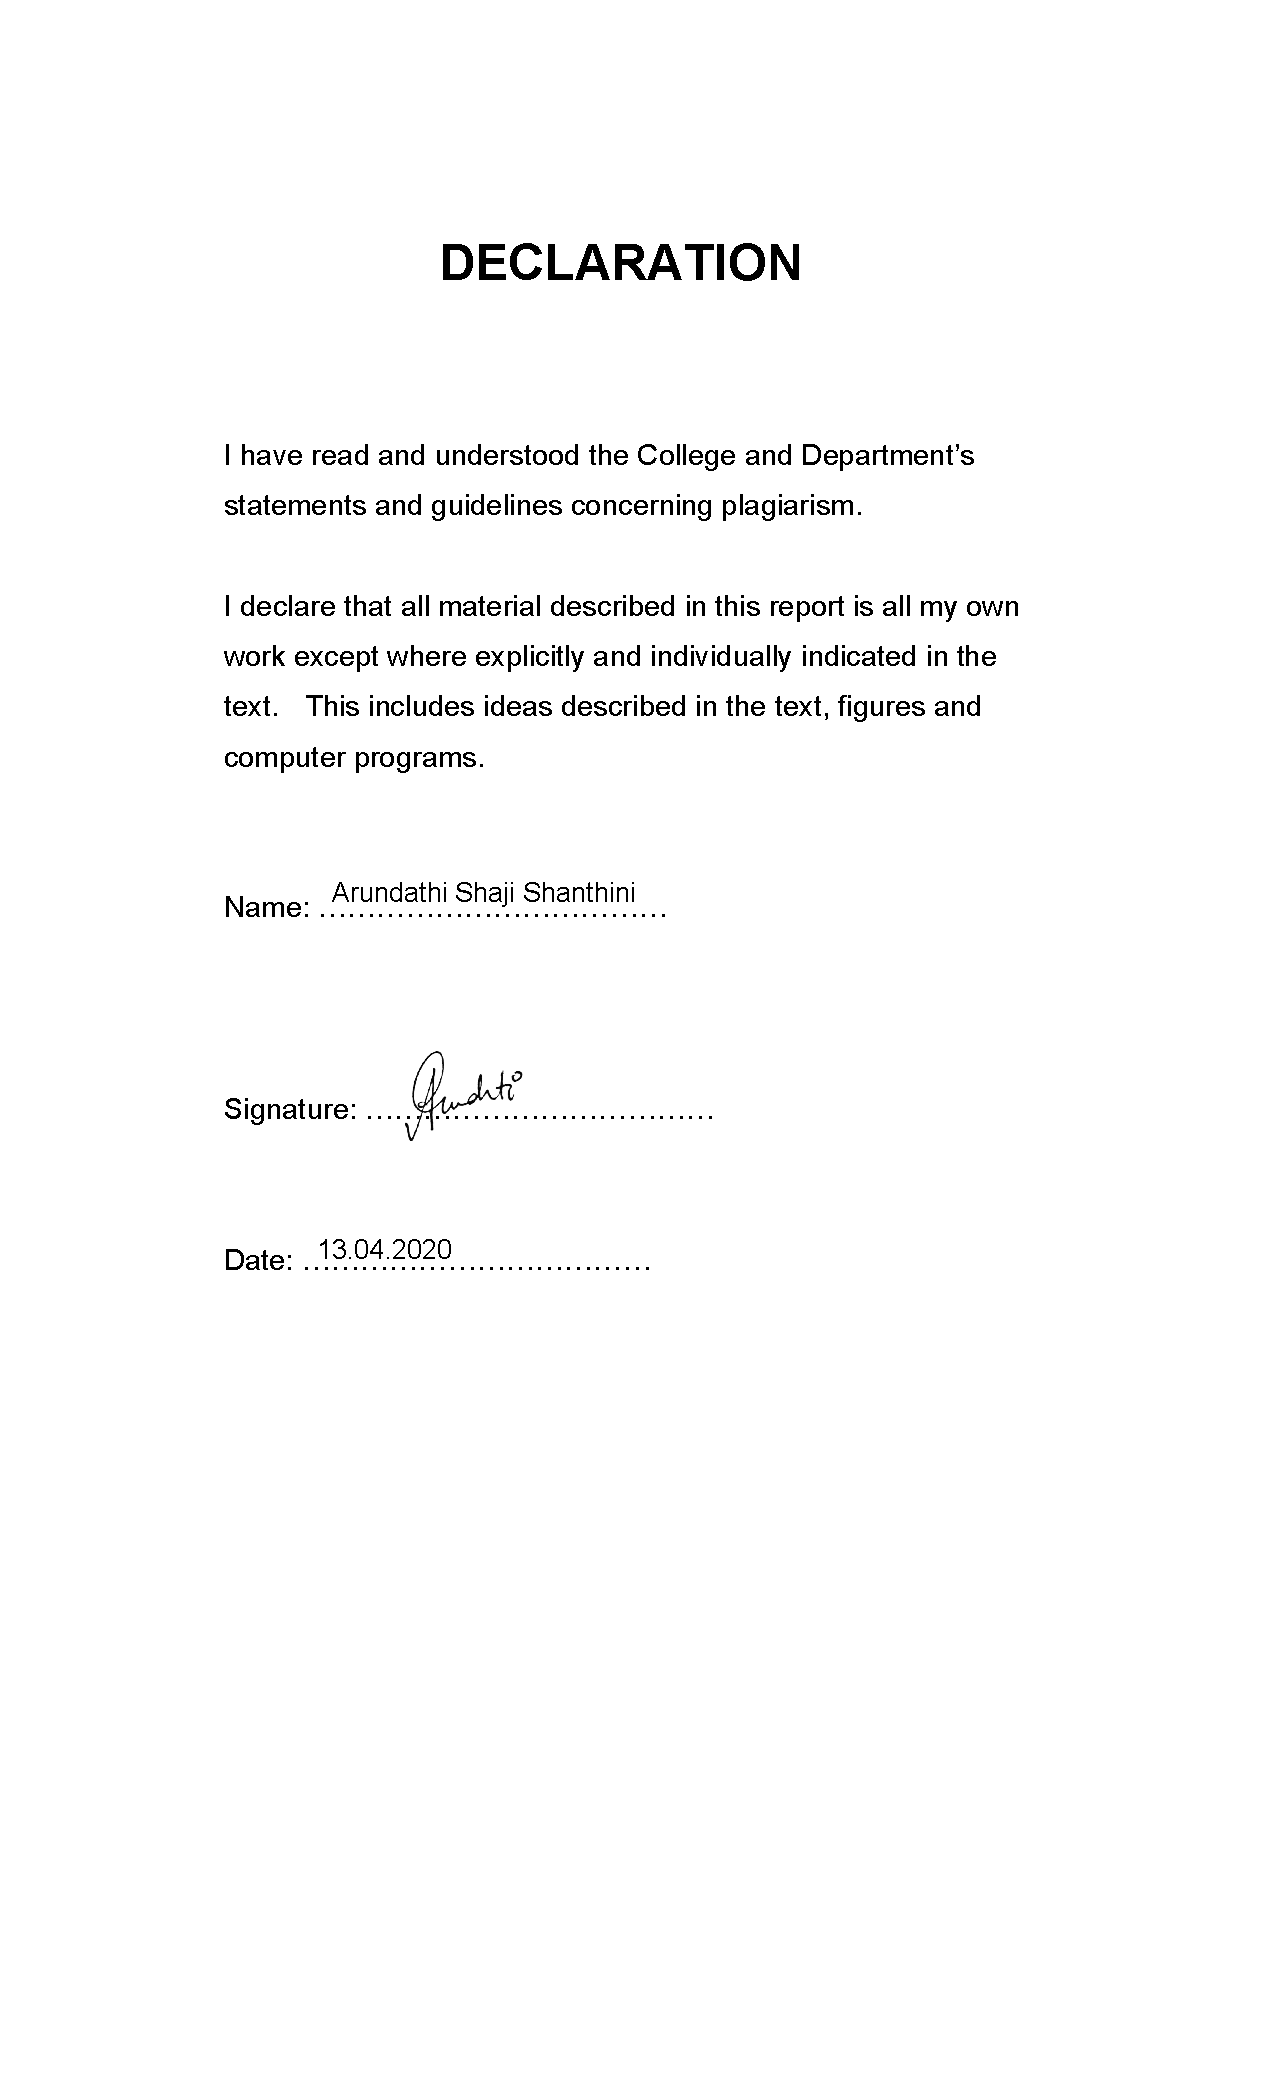
\includepdf[page=-]{files/Declaration}

\tableofcontents

\pagebreak

%%%%%%%%%%% ABSTRACT %%%%%%%%%%%%%%%%%
\begin{abstract}
    Cable-driven continuum robotic arms are widely used because of its
    high accessibility and manoeuvrability properties. It also has the ability to perform dexterous in-situ tasks even in confined and hazardous spaces. However, for applications involving imaging/measurement tasks, precise trajectory tracking of the end-effector is essential. This project involves modelling this robotic manipulator and developing a potentially robust control configuration that ensures very low tracking error. For this, the kinematic and dynamic model of the system was developed, cross-validated and implemented in Simulink. Then, a baseline control system design was proposed. However, due to time constraints, only implementation of the the proposed control scheme could be achieved. Improving the results from the controller for the dynamic model and the analysis of its robustness remains work to be undertaken further.
\end{abstract}
%%%%%%%%%%%%%%%%%%%%%%%%%%%%%%%%%%%%%%

%%%%%%%%%%% INTRODUCTION %%%%%%%%%%%%%%%%%
\chapter{Introduction}

Industrial robots that perform repetitive dexterous tasks have been around for quite some time. Over the years, these industrial robots have developed from being just command following, space-occupying large devices to systems that have better manoeuvrability, intelligence and accessibility properties, enabling it to  perform a myriad of operations. Expanding a robot's taskspace by improving the manoeuvrability of a robot has been of great interest and over the past decade a lot of interest has grown towards bio-mimetic or bio-inspired systems to achieve this.

Bio-inspired robotic systems implement concepts of locomotion inspired from nature onto robotic systems. This involves studying concepts of locomotion from nature and implementing that into robotic systems. One such kind of bio-inspired system is a snakebot. The locomotion achieved by snakes is highly desirable because of its accessibility and manoeuvrability properties which means that snakes can access confined spaces and manoeuvre through different kinds of terrain. The undulatory motion of snakes enables them to traverse through terrains where legged robots usually fail. Additionally, it is known that some snake gaits makes it possible for them to swim, while some snakes can even fly \cite{pettersen2017snake}. Such manoeuvrability of snakes have generated a lot of interest in wanting to study the different gaits of a snake and developing a mathematical model so that the motion can be mimicked. Successful prototypes of such robots have been proven to be very useful in a wide range of applications such as disaster management (it can collect data and images from inaccessible areas at search and rescue sites), industrial inspection - like subsea operations, aircraft wing inspection, military reconnaissance etc. Fig. \ref{snakebots-fig} shows some of the different kinds of snakebots that have been developed over the years by different research groups around the world. Some of these are amphibious snakebots which means that they can operate in both on land and under water.
\begin{figure}[h]
	\centering
	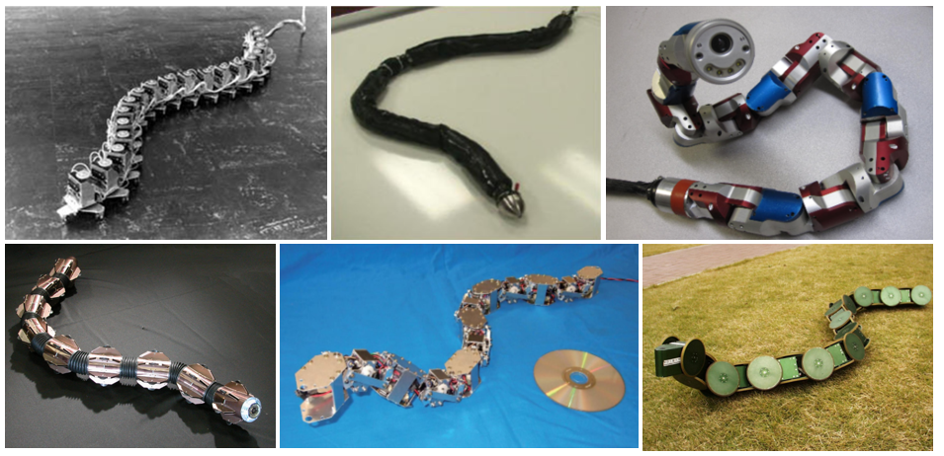
\includegraphics[width=\textwidth]{images/Intro-pic1.png}
	\caption{\textit{This picture shows some of the various kinds of snakebots that has been developed over the years. It shows examples of wheeled, wheel-less and amphibious snakebots that are used for varied operations. The pictures were sourced from a review on snakebots by Liljeb{\"a}ck P. et.al. \cite{liljeback2012review}}}
	\label{snakebots-fig}
\end{figure}

While Fig. \ref{snakebots-fig} shows different examples of ground-hugging, vertebrae structure type snakebots that were studied and developed for their ability to propagate through challenging terrains, there are also studies around using the body-structure of snakes as an inspiration for developing wire-driven “invertebrate like” continuum robotic arms which have better flexibility and manoeuvrability. \textit{Continuum robotic arms} are continuously curving manipulators that can be used to manoeuvre through confined and inaccessible places and can be made to perform dexterous in-situ tasks. In comparison to a normal non-redundant robotic manipulator higher degree of freedom means that the robot will have a bigger task space for manipulation. Generally, the hyper-redundancy is achieved in the design through springs or cables. In the robotic manipulator studied by this project, the joints of the manipulator are driven by cables (wire ropes).

\textit{Cable-driven Hyper-redundant Manipulator (CDHRM)} is a continuum robotic arm that is driven by wire-ropes and can be used in various applications involving service operations in confined spaces and hazardous environments, close range measurements, imaging etc. Generally, there are 2 types of CDHRM which differ in their design. Type I or multi-segmented elastic CDHRM has multiple segmented backbone that are controlled by cables that run through the robot. Type II or fully-constrained rigid CDHRM has multiple rigid links attached to each other through universal joints in between with cables running through designated holes along the periphery of the shell of the link. Fig. \ref{Type2-CDHRM} shows a Type II CDHRM which is similar to the system being studied by this project. 

\begin{wrapfigure}{r}{0.6\textwidth}
	\centering
	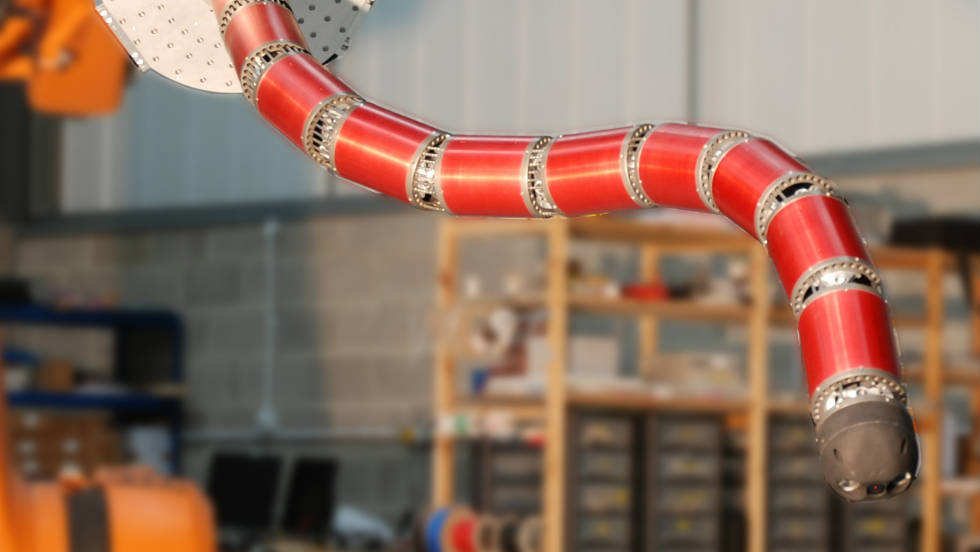
\includegraphics[width=0.6\textwidth]{images/CDHM.jpg}
	\caption{\textit{A cable-driven robotic snake arm developed by OC Robotics \cite{CNNarticle}}}
	\label{Type2-CDHRM}
\end{wrapfigure}

While such a CDHRM comes with extra manoeuvrability and accessibility properties, one of the other main advantages of this particular kind of robotic arm is that, it has no electronics in the robot itself. All of the electronics associated with the robot is located in the base to which the first joint of the arm is fixed. This makes it possible for the robot to access even hazardous environments without any risk of damage to the robot (except minor structural damage) or hindrance to its operation. This is desirable as this feature of the structural design makes the robot qualify some of the safety considerations for industrial application and hence makes risk assessments for systems with such a structure easier. 

\section{Project Description and Motivations}

A key area for research undertaken by UCL Robotics addresses one of the technology challenges of Robotics and Autonomous Systems (RAS) which is - “Robotic Teleoperation for Multiple Scales”. Under this challenge, attempts have been made to use photogrammetry techniques for the structural testing of aircraft wing of an Airbus by measuring the shape and dimensions of aerodynamic surfaces \cite{shortis2016photogrammetric}, and the six degrees of freedom (6DoF) position and orientation of aerospace models to study its structural dynamics and aerodynamic forces.

Photogrammetry is one of the optical metrology methods that obtains measurements of physical objects and/or their environment with a high accuracy through the process of capturing or recording photographic images and patterns of electromagnetic imagery and analysing it to measure and interpret reliable information of the object and environment under consideration. There are many variants of photogrammetry. The photogrammetry technique being studied at UCL involves the measurement of shape of aerodynamic surfaces and the six degree of freedom (6DoF) position and orientation of aerospace models.

Photogrammetry for aerospace models requires a non-contact, non-intrusive, accurate and reliable technique with a high sample rate. Within this study, the measurement of aerospace models in wind tunnel test sections are novel and for such a specialised measurement, close range photogrammetry is well suited. Currently off-the-shelf-digital cameras are used from different fixed positions to simultaneously capture/record images, however this has limitations and makes close-range photogrammetry difficult.

The proposed solution to this involves using a snake-arm that uses optical metrology techniques for aerodynamic surfaces. For this study, there is a physical snake-arm on-site at Here East and this project proposed is aligned to the modelling and control research effort being developed for this snakebot.

The snake-arm robot at Here East has been provided by OC Robotics. It is classified as Series II X125 snake-arm robot. The robot was specifically designed for the robotic deployment of photogrammetry capability for measurement and inspection of cluttered or confined 3D environments. This snake-arm is the unsleeved version of the Series II X125. It can potentially achieve up to 225 degrees of cumulative bend \cite{OCRobotics_Series_II_Webpage} and has an independently controlled tip. Currently, it simply uses a nose following control technique to reach to the desired final position.  The head of the snake can have different payloads attached to it. Unlike other versions of this series of snake-arms, the tethered end of this robot rests on a platform that can move forward and backward as required.

This project involves modelling this physical snakebot and understanding the end-effector pose control requirements for performing automated close-range optical metrology operations (specially photogrammetry). Once the control requirements are defined and the control strategies are realised, then the project aims to develop a robust control system that can perform measurements in various scenarios including measurements in wind tunnels. The control system configuration will be simulated, and the results obtained will be analysed and improved over the course of the project. Depending on the metrology technique adopted and in the case of using the robot to perform dexterous tasks such as maintenance of the structure, the payload attached to the head of the robot is subject to change. Significant external disturbances may be acting on the robot as well, especially in cases where the robot is performing dexterous tasks or is in environment with considerable disturbances like in a wind tunnel. Therefore, the robustness of the system will be tested using change in mass of head node and/or external disturbances acting on the snake-arm.

\section{Literature Review}

On investigating some of the literature around snakebots it can be seen that many different kinds of approaches were adopted towards developing snakebots. Earlier in the decade, wheeled snakebots were being developed a lot more than wheel-less snakebots. \cite{saito2002modeling} discusses some of the very early work done on wheeled snake robots and gives more insight to the motivations for study of wheel-less snake robots. Hirose S. \cite{1521742} through his work came up with the mathematical equation that represented the shape that the snake assumes to propagate forward. He introduced the concept of serpenoid curve which has been extensively used by other research groups till date to develop a mathematical model for the serpentine locomotion of snakes. Work done by Pettersen, K. Y. et. al. \cite{pettersen2017snake} also provides a very detailed insight into the research around snake robots and discusses the mathematical model, design and control system used for productionising amphibious snake robots. This source is an excellent summary of the history and study of snake robots. While most of these papers discuss wheel-less snake robots with rigid links, \cite{Zhou2018AnalysisOU} discusses how wire-driven "invertebrate like" continuum arm can have better flexibility and accessibility properties. A detailed review on the work done around continuum robots has also been published by Singh P. K. et. al.\cite{singh2014continuum}.

Since, the system under consideration is specifically that of the OC Robotics snake arm, materials published by the founders Graham A. and Buckingham R. were of immense interest. Even though material directly related to the robot or its technology could not be found, \cite{RN4,RN5,RN42} by these authors were a good introduction to their work on snake arms and the bigger context of the varied applications of such robots. The slides in \cite{RN42}, also discussed the main features of  snake arm robots.

Given that the system was identified as a wire rope driven, hollow core structure with passive revolute joints connecting the links to each other, attempts were made to identify literature around modelling of a similar system. The work of Jones B. et al. \cite{RN2} (dated 2006) has been cited in most papers. His work on kinematics for multi-section continuum robots seems to be the inspiration for most of the work around continuum snake arm robots. The works of Li Z. et al. \cite{RN8,RN7,RN15,RN21} discusses how the skeleton of the robot is inspired from the skeleton of a snake and the idea of a the cable driven structure is inspired from the muscle arrangement in the tentacle of an octopus. Even though across various papers their work discusses the kinematic model of the snake arm robot, they do not discuss much about the dynamic model and control of the system. The references \cite{RN35,RN31,RN29,RN30} represents the OC robotics snake arm the most. The system described by these papers uses a cable-driven hyper-redundant manipulator (CDHRM) in which the cables are controlled at the base with maxon motors exactly like the snake arm at Here East. The papers published by Tang L. et al. \cite{RN35,RN31} describes the design, motion planning and path tracking of the snake-arm.  Most of the literature related to the CDHRM refers a detailed study and experiments based on its kinematic model. \cite{RN29,RN31} discuss the kinematic model in detail. The simulation and a path planning method for the CDHRM using the kinematic model is given by \cite{RN35}. The main challenge in developing a kinematic model for this manipulator is around the inverse kinematic relationship. The forward kinematic model can have infinite solutions, is non-homogenous and has a non-linear relationship. \cite{RN2} proposes a numerical solution to this problem whereas other sources propose more efficient geometrical methods \cite{chirikjian1994modal} or complex learning methods\cite{giorelli2013feed}. However, the work of Xu W. et al \cite{RN30} dated 2018, remains the most suitable reference found so far as it discusses the dynamic model and control of the cable-driven snake arm in great detail. 

\section{Aims and Objectives}
\label{objectives}
The aim of this project is to contribute to the modelling and control effort around the snake-arm at Here East by developing and implementing a mathematical model and testing a control system configuration suitable for the task.

The main objectives of the project are:
\begin{itemize}
	\item \textbf{Develop and implement a mathematical model that best represents the snake-arm at Here East:} The main aim of the project is to develop and implement a mathematical model that best represents the system using Simulink. The model will be then tested to ensure that its behaviour is as expected and represents the snake-arm well.
	\item \textbf{Design and test control strategies that will help control the path followed by the arm during the metrology task:} The next objective is to define control requirements for the automation of the optical metrology process and design control strategies that performs the operation with the required accuracy. Through iterative testing, the model will be improved over the course of the project till satisfactory results are obtained.
	\item \textbf{Analyse the robustness of the control system configuration developed by running experiments with varied physical parameters:} The project also aims to investigate the robustness of the system since it is expected to work in environments with varied conditions where external disturbances affecting the arm’s propagation might be considerable. It is also expected that depending on the technique adopted for the optical metrology different payloads may be attached to the head of the snakebot. The payload may also change in mass especially in occasions when improvements have been made to the same metrology technique under consideration. Therefore, the robustness of the system under the influence of change of mass of the head and the external disturbances will be investigated through experiments in the simulation software.
\end{itemize}

The following chapters discuss the theory, proposed solution and the results as obtained for the work undertaken as part of this project. Chapter 2 discusses the kinematic and dynamic model equations and its brief derivation. Chapter 3 discusses the attempt at implementation of these on Simulink and the proposed control scheme. Chapter 4 presents the results obtained and finally, Chapter 5 concludes the results observed, problems faced etc.

%%%%%%%%%%%%%%%%%%%%%%%%%%%%%%%%%%%%%%

\chapter{Mathematical Modelling}

The first step towards simulation of a control scheme for any plant involves developing/identifying a suitable mathematical model that represents the physical system (the plant). This chapter discusses briefly the derivation of the mathematical model of the snake arm under consideration. For this, first the mechanical design of the system was understood. Given the unique structural design of the CDHRM, it was realised that a kinematic model had to be developed in order to map the reference value (the end-effector position) to the actuator variable (motor angle of rotation) that can be controlled and vice versa. In the later half of the chapter, the derivation of the dynamic model (the plant block) representing the system has been discussed.

\section{Understanding the system}
To find the most suitable mathematical model for the snake-arm, a clear understanding of the system itself was to be established. This also included identifying the actuators that drive the system and understanding what can be controlled. This was essential to determine what parameters and system variables were required to be calculated in order to derive the mathematical model and to also understand exactly what can and cannot be controlled.

The videos that have been made available by OC Robotics \cite{OCRobotics_videos_1, OCRobotics_videos_2, OCRobotics_videos_3, OCRobotics_videos_4}, helped to understand the snake-arm and its capabilities to an extent. The snake-arm developed by OC Robotics is a hollow core structure with a fixed number of links. Each joint is driven by 3 wire ropes (big stainless steel cable ropes) that runs through the holes in the shell of the link at equidistant points from each other, parallel to the surface of the shell of the link. \cite{OCRobotics_article} (as can be seen in Fig. \ref{base-pic}). The cables are controlled by 27 or more motors in the base \cite{OCRobotics_videos_2} using maxon motors as it offers higher power density. All the electronics associated to the robot including the control systems are located at the base of the robot. This means that the robot can easily operate even in hazardous environments. The nose of the snake arm can accommodate different payloads and it also has a hollow core, which allows cables, hoses or any other equipment required by the specific payload to be routed through the centre of the snake arm.
\begin{wrapfigure}{r}{0.5\textwidth}
	\centering
	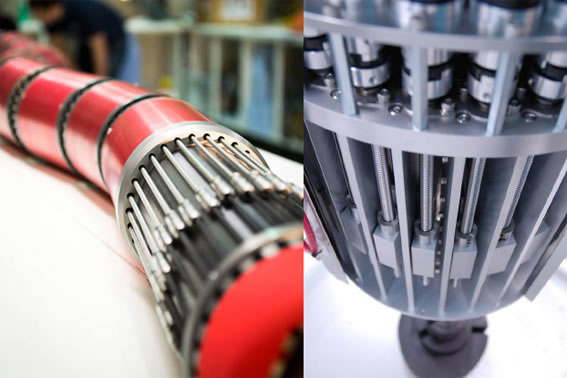
\includegraphics[width=0.5\textwidth]{images/maxon-motors.jpg}
	\caption{\textit{The figure showing the maxon motors at the base to which the wire-ropes are attached (right) and the transmission system (left) that converts the rotational motion of motor to translational motion of the wire-ropes. \cite{CNNarticle}}}
	\vspace{-15pt}
	\label{base-pic}
\end{wrapfigure}

In the video for Maxon Motors \cite{OCRobotics_videos_2}, Graham A. also talks about the unique nose following property of the snake arm robot and how it is easily controlled using a proprietary software developed by OC Robotics. 
From these information, it can been safely concluded that the system closely represents a cable-driven hyper-redundant manipulator (CDHRM) and so the mathematical model developed for the robot was derived mainly, with help of the following literature \cite{RN30, RN31, RN29} around modelling of a CDHRM. Kinematic modelling and Dynamic modelling have both been studied for the CDHRM. While kinematic modelling of the CDHRM has been thoroughly studied, there are only very few papers that discuss dynamic modelling.

\section{Model Preliminaries \normalsize{(Structural Design Description)}}

Consider a CDHRM snake-arm with \textbf{N universal joints} and hence has \textbf{N+1 links}. The length of each link is $l_{link}$, the distance between 2 joints is $a$ and the distance between the two links is $2d$. Given the structural design, we can say that $l_{link}=a-2d$. Each universal joint consists of 2 revolute joints connected via a common lumen which facilitate either a pitch or yaw rotation which imparts each joint 2 degrees of freedom (DoF). This means that in total the snake arm has \textbf{2N DoF}. 
\begin{figure}[h]
	\centering
	\includegraphics[width=\textwidth]{images/CDHRM System.png}
	\caption{\textit{A figure showing the structural design of a CDHRM. Adapted from \cite{RN29}}}
	\label{CDHRM-structure}
\end{figure}

Every link has an identical structure but is connected at 90\textdegree with respect to each other. A link consists of a hollow cylindrical shell with two identical disks. The disk extensions from 2 links join in the centre onto a common lumen to form a universal joint. The links are arranged such that the joints in between forms an alternate pitch-yaw formation as described below.
\begin{wrapfigure}{b}{0.4\textwidth}
	\centering
	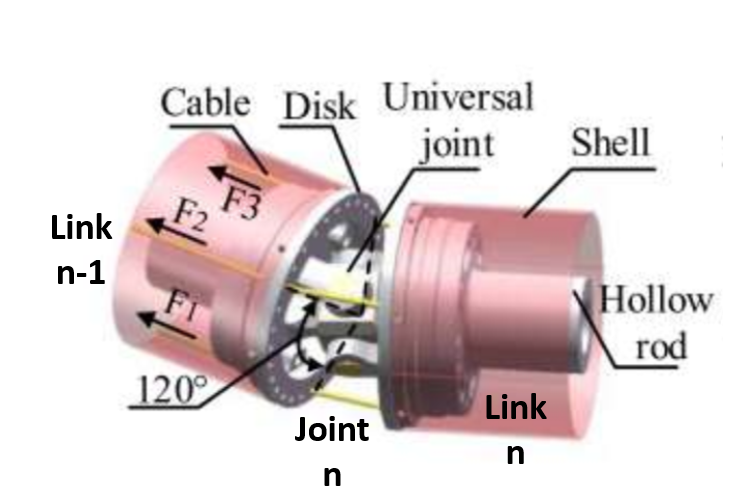
\includegraphics[width=0.4\textwidth]{images/cable_in_case.png}
	\caption{\textit{This figure shows the cables driving the joints are placed at equidistant positions. Taken from \cite{RN30}}}
	\vspace{-40pt}
	\label{cable-pos}
\end{wrapfigure}
\begin{center}
	Fixed Base --- (Pitch-Yaw) --- (Yaw-Pitch) --- (Pitch-Yaw)\ldots\ldots) --- Nose link
\end{center} 

For a given joint $n$ ($n \in {1,2,\ldots,N}$), the disc attached to link $n-1$ is called the \textbf{distal disc} and the disc attached to link $n$ is called the \textbf{proximal disc}. Given this notation, note that as depicted in Fig. \ref{CDHRM-structure} a given link number $i$ can be denoted such that $i \in \{0,1,2,\ldots,N\}$ where, base is link $0$ and the nose is link $N$.


Each joint is driven by three cables placed at equidistant angles (i.e. at 120\textdegree) from each other. Therefore, there are $3N$ holes on each disc through which the cables are routed. Out of the $3N$ cables, each link will have a total $3(N-n+1)$ cables routed to it such that $3(N-n)$ cables pass through and $3$ cables terminate at the proximal disc of that link n. For a given joint $n$, cables $C_{3n-2}$,$C_{3n-1}$ and $C_{3n}$ drive joint $n$ and terminate at the proximal disc of the link $n$ as can be seen in Fig. \ref{cable-pos}. In the following sections, a cable will be represented by the notation, $C_{k}$ where, $k \in \{1,2,3,....,3N\}$.

\section{Kinematic Model}

To establish the relationship between the task space and the control space a kinematic model was required. The kinematic model here finds the relationship between the angle of rotation of the motor and the end-effector pose of the snake-arm. The conversion from the control space to task space and vice versa involves a multi-level mapping through relationships between parameters in different spaces. This is because unlike in common robotic manipulators, the actuators do not directly control the joint angles. In the case of a CDHRM, the motors drive the cables, and the cables drive the joint. This multi-level mapping from the control space to the task space is depicted in Fig. \ref{kinematic map} below.
\begin{figure}[h]
	\centering
	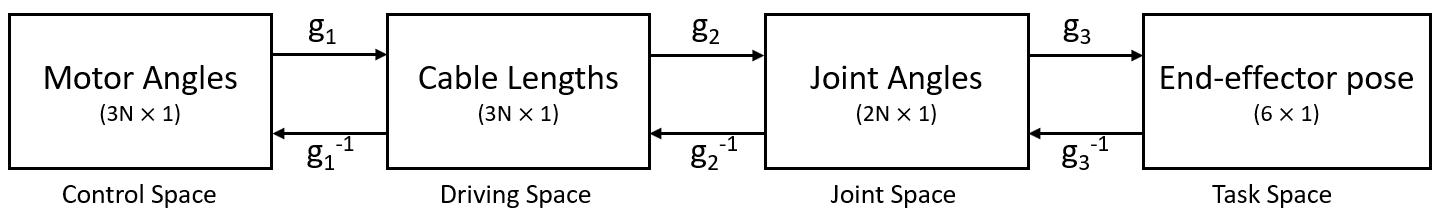
\includegraphics[width=\textwidth]{images/Kinematics-mapping.png}
	\caption{\textit{This picture shows the various mapping relationships required between different spaces to derive the relationship between the angle of rotation of the motor and the end-effector pose of the snake-arm}}
	\vspace{-30pt}
	\label{kinematic map}
\end{figure}

\subsection{Motor Angle of Rotation - Cable Length Kinematics}
\subsubsection{Motor Angle of Rotation \textbf{$\longrightarrow$} Cable Length (Forward Kinematics)}
The rotation of the motors at the base are transmitted as translational motion causing a change in length of the cable driving the robotic arm. For a given change in angle of rotation of the motor the change in cable length (the translational distance travelled) can be calculated as \cite{derbel2019new}:
\begin{equation}
\label{eq:g1}
\Delta L_{k} = k_{trans}\sqrt{(r_{drum})^2 + (\frac{p}{2 \pi})^2} \times \Delta \theta_{motor,k}
\end{equation}
where,
\begin{itemize}
	\renewcommand\labelitemi{--}
	\item $\Delta L_{k}$ = Change in length of cable number $k$ 
	\item $\Delta \theta_{motor,k}$ = Angle of rotation of the motor
	\item $k_{trans}$ = Transmission Ratio
	\item $r_{drum}$ = Radius of the Drum
	\item $p$ = Pitch of the Drum
\end{itemize}
\subsubsection{Cable Length \textbf{$\longrightarrow$} Motor Angle of Rotation (Inverse Kinematics)}
Equation (\ref{eq:g1_inv}) is the inverse kinematic relationship between the motor angle of rotation and cable length ($g_{1}^{-1}$ as per Fig. \ref{kinematic map}). From this the forward kinematic relationship($g_{1}$ as per Fig. \ref{kinematic map}) between the motor angle of rotation and cable length can be derived as:
\begin{equation}
\label{eq:g1_inv}
\Delta \theta_{motor,k} = \frac{\Delta L_{k}}{k_{trans}\sqrt{(r_{drum})^2 + (\frac{p}{2 \pi})^2}}
\end{equation}

\subsection{Cable Length - Joint Angle Kinematics}
\subsubsection{Joint Angle \textbf{$\longrightarrow$} Cable Length (Inverse Kinematics)}
To derive the relationship between the cable length and the joint angles, three reference frames $\{P_n\}$,$\{U_n\}$ and $\{D_n\}$ must be defined at each universal joints as seen in Fig. \ref{ref-frames}.

\begin{itemize}
	\item The reference frame $\{U_n\}$ is defined such that its origin ($O_U$) corresponds to the centre of the joint. $X_U$ is defined parallel to $\zeta_P$ and $Y_U$ is defined parallel to $\zeta_D$. $Z_U$ is then defined using right-hand thumb rule.
	\item The reference frame $\{P_n\}$ is defined such that its origin ($O_P$) corresponds to the centre of the proximal disk. $Z_P$ is normal to the proximal disc and $X_P$ is parallel to $\zeta_P$. $Y_P$ is then defined using right-hand thumb rule.
	\item The reference frame $\{D_n\}$ is defined such that its origin ($O_D$) corresponds to the centre of the distal disk. $Z_D$ is normal to the distal disc and $Y_D$ is parallel to $\zeta_D$. $X_D$ is then defined using right-hand thumb rule.
\end{itemize}

where, $\zeta_P$ and $\zeta_D$ represents the axis of rotation of the joint attached to the proximal and distal discs respectively.
This means that by definition we have the relationship: $O_{P,n}O_{U,n}=O_{U,n}O_{D,n}=d$
\begin{figure}[H]
	\centering
	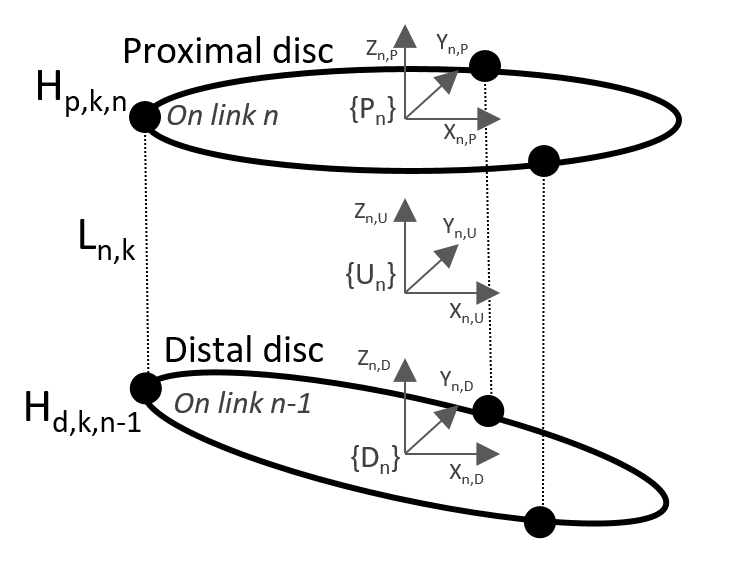
\includegraphics[width=0.5\textwidth]{images/Refrence_frames.png}
	\caption{\textit{This diagram shows the different reference frames that were defined}}
	\label{ref-frames}
\end{figure}

The transformation matrix from $\{D_n\}$ to $\{P_n\}$ can be defined as: 
\begin{equation}
\begin{aligned}
^DA_P&=^DA_U \times ^UA_P \\ 
&= \begin{bmatrix}
\cos{\phi_{p,n}}&0&\sin{\phi_{p,n}}&d\sin{\phi_{p,n}}\\
\sin{\phi_{p,n}}\sin{\phi_{d,n}}&\cos{\phi_{d,n}}&-\sin{\phi_{d,n}}\cos{\phi_{p,n}}&-d\sin{\phi_{d,n}}\cos{\phi_{p,n}}\\
-\cos{\phi_{d,n}}\sin{\phi_{p,n}}&\sin{\phi_{d,n}}&\cos{\phi_{d,n}}\cos{\phi_{p,n}}&d+d\cos{\phi_{p,n}}\cos{\phi_{d,n}}\\
0&0&0&1\\
\end{bmatrix}\\
\end{aligned}
\end{equation}

\begin{wrapfigure}{t}{0.4\textwidth}
	\centering
	\vspace{-50pt}
	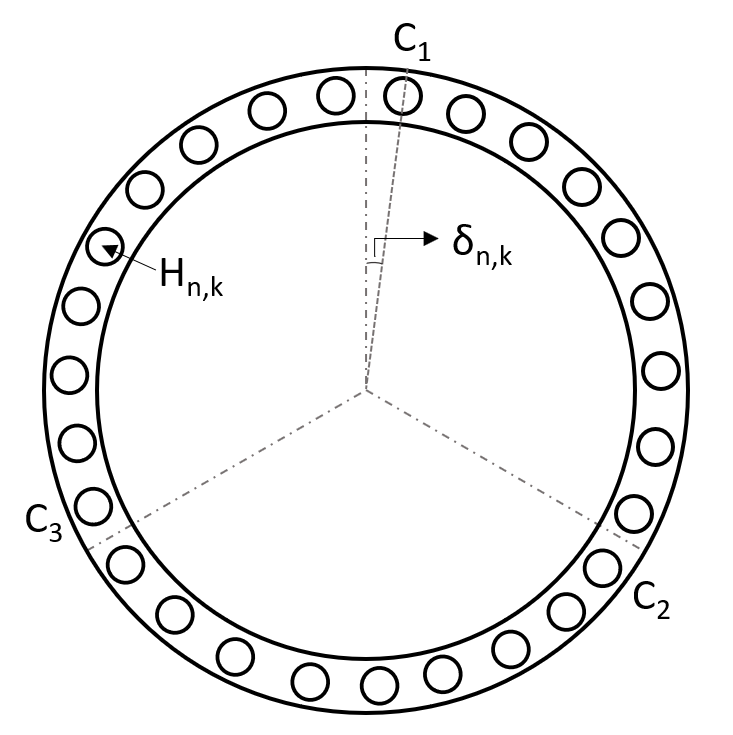
\includegraphics[width=0.4\textwidth]{images/hole_positions.png}
	\caption{\textit{This diagram shows the angular positions of the holes on a disc.}}
	\label{hole-pos}
\end{wrapfigure} 
As can be seen from Fig. \ref{ref-frames} the length of the cable between 2 discs can be derived as:
\begin{equation}
\label{len_joints}
l_{k,n}= \lvert\lvert ^DA_P^PH_{p,k,n} - ^DH_{d,k,n-1}  \rvert\rvert
\end{equation}
such that,
\begin{equation*}
^PH_{p,k,n}=\begin{bmatrix}
r\cos{\delta_{n,k}}\\
r\sin{\delta_{n,k}}\\
0\\
\end{bmatrix};  \\
\end{equation*}

\begin{equation*}
^DH_{d,k,n-1}=\begin{bmatrix}
r\cos{\delta_{k,n-1}}\\
r\sin{\delta_{k,n-1}}\\
0\\
\end{bmatrix} 
\end{equation*}

where, $^PH_{p,k,n}$ and $^DH_{d,k,n}$ is the vector defining the position of the hole on the proximal and distal disc respectively w.r.t their local reference frame.

The angular position of these holes as seen in Fig. \ref{hole-pos} can be calculated as:
\begin{equation}
\label{delta-hole-pos}
\delta_{n,k} =
\begin{cases}
\dfrac{120^{\circ}}{(N+1)} \times M +120^{\circ}(k-1) - 3^{\circ} &; \hspace{1mm}  \text{n = odd}   \\
\dfrac{120^{\circ}}{(N+1)} \times M +120^{\circ}(k-1) + 87^{\circ} &; \hspace{1mm}  \text{n = even}
\end{cases}
\end{equation}
where,
\begin{itemize}
	\renewcommand\labelitemi{--}
	\item $M = floor((k-1)/3)+1$ is the link at which cable $k$ terminates.
\end{itemize}
The total length of the cable $k$ can therefore be written as:
\begin{equation}
\label{len_total}
L_k= M\hspace{1mm}l_{link} + \sum_{j=1}^{M}l_{j,k}
\end{equation}
Therefore,  equations (\ref{len_joints}) and (\ref{len_total}) define the inverse kinematics relationship between the joint angles and the cable lengths ($g_{2}^{-1}$ as per Fig. \ref{kinematic map}).

\subsubsection{Cable Length \textbf{$\longrightarrow$} Joint Angle (Forward Kinematics)}
\label{numerical-case-1}
We know that for a given joint $n$, cables $3n-2$,$3n-1$ and $3n$ drive that joint. Therefore, considering equation (\ref{len_joints}) to be a function of $\phi_p$ and $\phi_d$ we know there exists a relationship:
\begin{equation}
\begin{bmatrix}
l_{n,3n-2}\\
l_{n,3n-1}\\
l_{n,3n}\\
\end{bmatrix} =
\begin{bmatrix}
f_{n,3n-2}(\phi_{p,n},\phi_{d,n})\\
f_{n,3n-1}(\phi_{p,n},\phi_{d,n})\\
f_{n,3n}(\phi_{p,n},\phi_{d,n})\\
\end{bmatrix}
\label{function_of_l}
\end{equation}

From equation (\ref{function_of_l}), the differential equation can be derived as: 
\begin{equation*}
\begin{bmatrix}
dl_{n,3n-2}\\
dl_{n,3n-1}\\
dl_{n,3n}\\
\end{bmatrix} = J_{d}
\begin{bmatrix}
d\phi_{p,n}\\
d\phi_{d,n}\\
\end{bmatrix}
\label{differential_of_l}
\end{equation*}
where,
\begin{itemize}
	\renewcommand\labelitemi{--}
	\item $J_{d}$ = Jacobian matrix of $[f_{3n-2}(\phi_{p,n},\phi_{d,n}),f_{3n-1}(\phi_{p,n},\phi_{d,n}),f_{3n}(\phi_{p,n},\phi_{d,n})]^{T}$ w.r.t $[\phi_{p,n},\phi_{d,n}]^{T}$ given by, 
	\begingroup
	\renewcommand{\arraystretch}{1.5}
	\begin{equation*}
	J_{d} = 
	\begin{bmatrix}
	\dfrac{dl_{3n-2}}{d\phi_{p}} & \dfrac{dl_{3n-2}}{d\phi_{d}} \\
	\dfrac{dl_{3n-1}}{d\phi_{p}} & \dfrac{dl_{3n-1}}{d\phi_{d}}\\
	\dfrac{dl_{3n}}{d\phi_{p}} & \dfrac{dl_{3n}}{d\phi_{d}}
	\end{bmatrix}
	\end{equation*}
	\endgroup
\end{itemize}

Therefore, the forward kinematics relationship between the joint angles and the cable lengths ($g_{2}$ as per Fig. \ref{kinematic map}) can be numerically calculated as:
\begin{equation}
\begin{bmatrix}
\Delta \phi_{p,n}\\
\Delta \phi_{d,n}\\
\end{bmatrix}
= J_{d}^{+}
\begin{bmatrix}
\Delta l_{3n-2,n}\\
\Delta l_{3n-1,n}\\
\Delta l_{3n,n}\\
\end{bmatrix}
\label{g2}
\end{equation}
where,
\begin{itemize}
	\renewcommand\labelitemi{--}
	\item $J_{d}^{+}$= Moore-Penrose pseudo-inverse of $J$
\end{itemize}

However, the calculation of Jacobian matrix $J_{d}$ requires us to know $\phi_{p}$ and $\phi_{d}$ and for this problem they are unknown. Therefore, equation (\ref{g2}) has 3 equations with only 2 unknowns and the equations are non-linear about them. This makes the unknown variables difficult to
\begin{wrapfigure}{t}{0.6\textwidth}
	\centering
	\vspace{-15pt}
	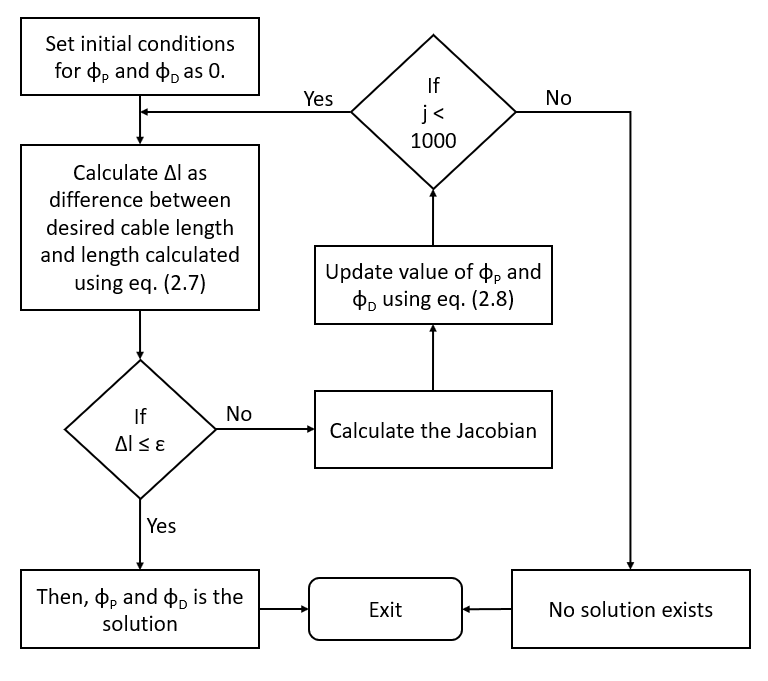
\includegraphics[width=0.6\textwidth]{images/Iteration_1.png}
	\caption{\textit{Flowchart showing the numerical iteration for Cable Length $\longrightarrow$ Joint Angle Kinematics}}
	\vspace{-40pt}
	\label{iteration-1}
\end{wrapfigure}
isolate and therefore the equations cannot be solved analytically. To solve this problem, \cite{RN30} proposes using a numerical iteration method that determines the least squares solution. 

This involves starting from the known initial condition when $\phi_{d}=0$ and $\phi_{p}=0$ given by:
\begin{equation*}
\begin{bmatrix}
f_{n,3n-2}(0,0)\\
f_{n,3n-1}(0,0)\\
f_{n,3n}(0,0)\\
\end{bmatrix} =
\begin{bmatrix}
2d\\
2d\\
2d\\
\end{bmatrix}
\label{initial-condition-iteration-1}
\end{equation*}
and the corresponding length $l_{k}$ is calculated. The difference between the desired and the calculated length is computed and is checked to see if it is within tolerance ($\epsilon$). Through each iteration the algorithm attempts to bring the calculated length value closer to the desired length value by using the error ($\Delta l$) to calculate the error in $\phi_p$ and $\phi_d$ and then updating the proposed solution with these errors. If no solution is found within tolerance before the maximum number of iterations is exceeded then the algorithm exits giving the message that "No solution could be found". Fig. \ref{iteration-1} presents the flow chart for this algorithm.

\subsection{Joint Angle - End-Effector Position Kinematics}
The problem of getting the end-effector position from joint angles is a very standard problem in robotics. The most commonly adopted approach involves using the Denavit-Hartenberg (D-H) parameters which provides a systematic approach to deriving the transformation matrix and hence the Jacobian matrix. However, the inverse kinematics approach does not have a standard approach and hence a numerical iteration method has been discussed.
\subsubsection{Joint Angle \textbf{$\longrightarrow$} End-effector Position (Forward Kinematics)}
\label{forward-jointangle} 
The first step towards deriving the forward kinematic relationship between the joint angles and end effector position is to define the D-H frames. Fig. \ref{kinematic-diagram} shows the kinematic diagram with the D-H frames defined as per rules. Based on this, the D-H parameters can be derived as per Table \ref{d-h-params}
\begin{figure}[H]
	\centering
	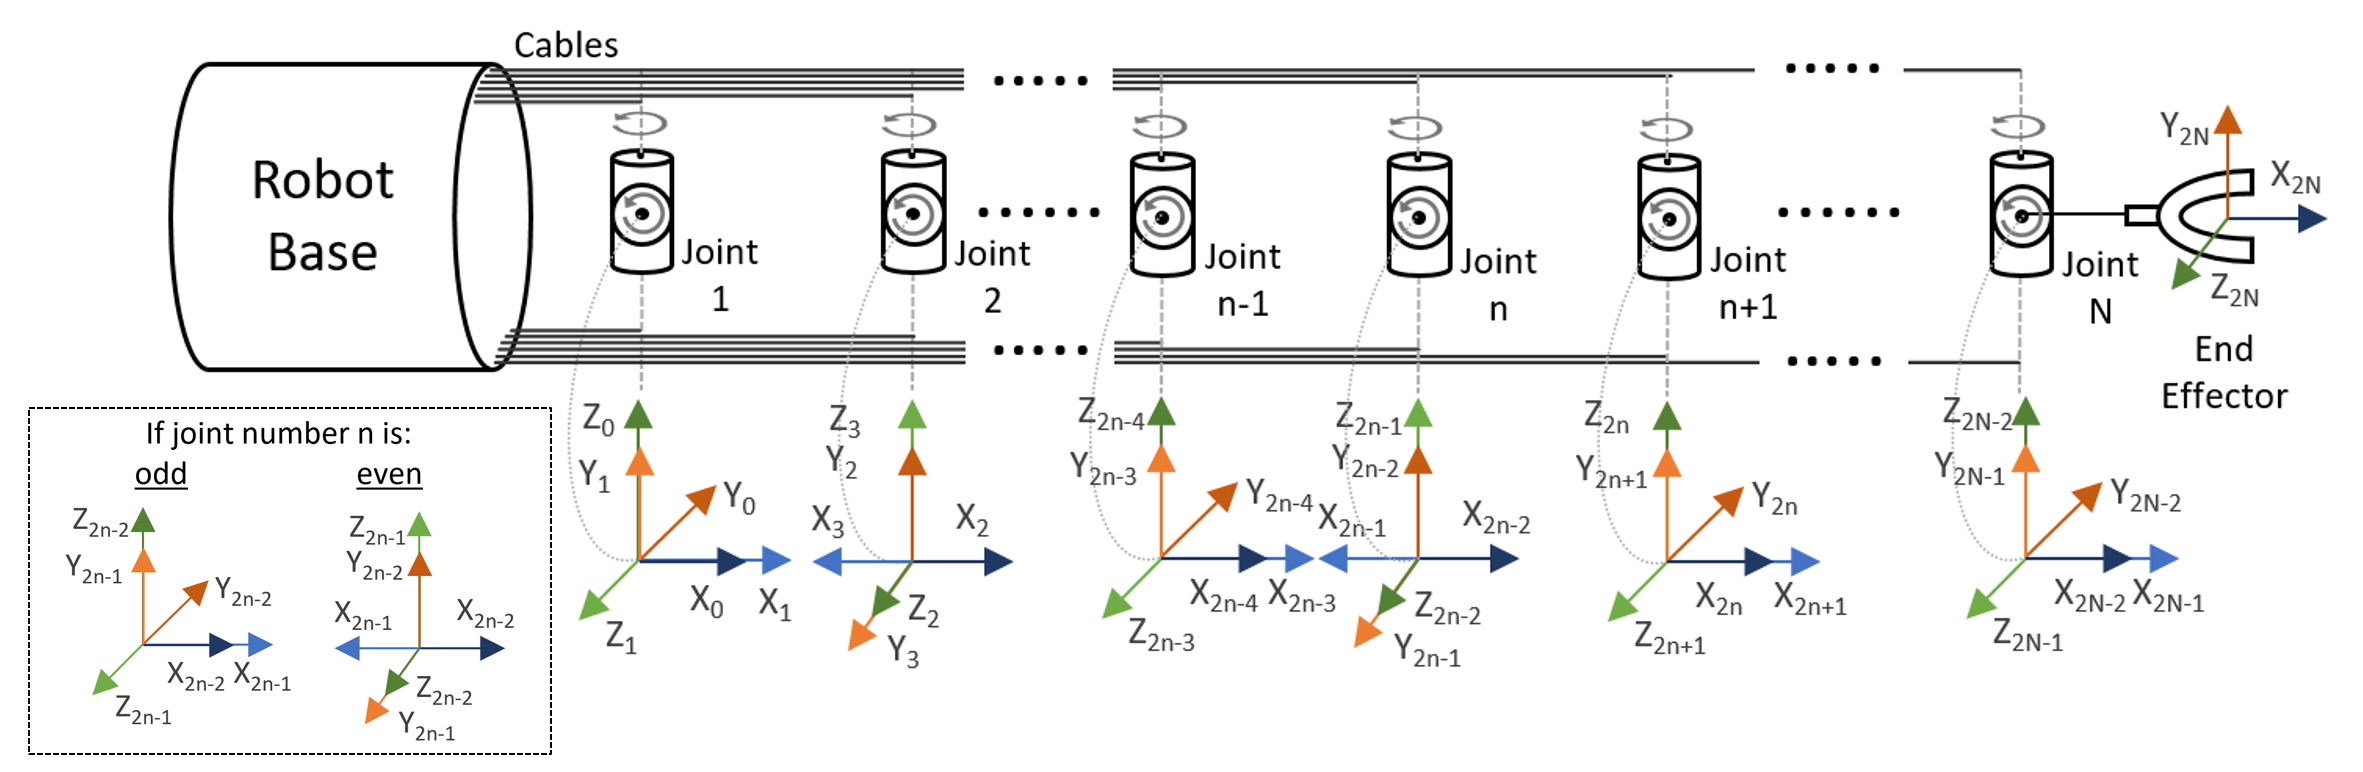
\includegraphics[width=\textwidth]{images/Kinematic-diagram.png}
	\caption{\textit{Kinematic diagram showing the universal joints as 2 revolute joints and shows the D-H frames.}}
	\label{kinematic-diagram}
\end{figure}

From the DH parameter table (Table \ref{d-h-params}), a row $n$ can be to calculate the homogenous transformation matrix for adjacent frames ${n-1}A_{n}$ as:
\[
{}^{n-1}A_{n}=
\begin{bmatrix}
\cos(\theta_{n}) & -\sin(\theta_{n})\cos(\alpha_{n}) & \sin(\theta_{n})\sin(\alpha_{n}) & r_{n}\cos(\theta_{n})\\
\sin(\theta_{n}) & \cos(\theta_{n})\cos(\alpha_{n}) & -\cos(\theta_{n})\sin(\alpha_{n}) & r_{n}\sin(\theta_{n})\\
0 & \sin(\alpha_{n}) & \cos(\alpha_{n}) & d_{n}\\
0 & 0 & 0 & 1\\
\end{bmatrix}
\]
\begin{wraptable}{r}{0.55\textwidth}
	\begin{tabular}{|c|c|c|c|c|}
		\hline
		\textbf{n}&\textbf{\straighttheta \textsubscript{n} (\textdegree)} & \textbf{\textalpha\textsubscript{n} (\textdegree)} & \textbf{r\textsubscript{n} (mm)} & \textbf{d\textsubscript{n} (mm)}\\
		\hline
		1&\straighttheta \textsubscript{1}&90&0&0\\
		2&\straighttheta \textsubscript{2}&0&a&0\\
		3&180+\straighttheta \textsubscript{3}&90&0&0\\
		4&180+\straighttheta \textsubscript{4}&0&a&0\\
		$\ldots$&$\ldots$&$\ldots$&$\ldots$&$\ldots$\\
		17&\straighttheta \textsubscript{17}&90&0&0\\
		18&\straighttheta \textsubscript{18}&0&a&0\\
		\hline
	\end{tabular}
	\caption{\textit{The DH Parameters}} 
	\label{d-h-params}
\end{wraptable}

This can then be used to derive the base to end-effector transformation matrix as: $^{0}A_{2N}= \hspace{1mm}^{0}A_{1}\cdot ^{1}A_{2}\cdot ^{2}A_{3}\ldots ^{2N-1}A_{2N} $,  which is a function of joint angles \straighttheta.

The differential kinematic equation for any robotic manipulator is given by:
\begin{equation}
\dot{x}_{end}= J \dot{\Theta}
\label{forward-joint-end}
\end{equation}
where,
\begin{itemize}
	\renewcommand\labelitemi{--}
	\item J = Jacobian Matrix
\end{itemize}
The Jacobian can therefore be calculated based on:
\begin{equation*}
J=
\begin{bmatrix}
J_v \\
J_{\omega}
\end{bmatrix}_{6 \times 2N} = 
\begin{bmatrix}
[J_{v1}]_{3 \times 1} & [J_{v2}]_{3 \times 1} & \ldots & [J_{v2N}]_{3 \times 1} \\
[J_{\omega 1}]_{3 \times 1} & [J_{\omega 2}]_{3 \times 1} & \ldots & [J_{\omega 2N}]_{3 \times 1}
\end{bmatrix}
\end{equation*}
where, \\
\begin{itemize}
	\renewcommand\labelitemi{--}
	\item $ J_{vi}= ^{0}R_{i-1} \begin{bmatrix} 0\\ 0\\ 1\end{bmatrix} \times (^{0}P_{2N} - ^{0}P_{i-1}) $
	\vspace{1mm}
	\item $ J_{\omega i}= ^{0}R_{i-1}\begin{bmatrix} 0\\ 0\\ 1\end{bmatrix} $
\end{itemize}
and, the rotational matrix ($^{n-1}R_{n}$) and position vector ($^{n-1}P_{n}$) can be taken from the homogeneous transformation matrix $^{n-1}A_{n}$ as:
\begin{equation*}
^{n-1}A_{n}=
\begin{bmatrix}
^{n-1}R_{n} & ^{n-1}P_{n} \\
0 & 1 \\
\end{bmatrix}
\end{equation*}
and, $^0A_{i-1}=\prod^{i-1}_{j=1} {}^{j-1}A_{i}$

\subsubsection{End-effector Position \textbf{$\longrightarrow$} Joint Angle (Inverse Kinematics)}

From equation (\ref{forward-joint-end}), we can derive the inverse relationship as:
\begin{wrapfigure}{b}{0.6\textwidth}
	\centering
	\vspace{-2mm}
	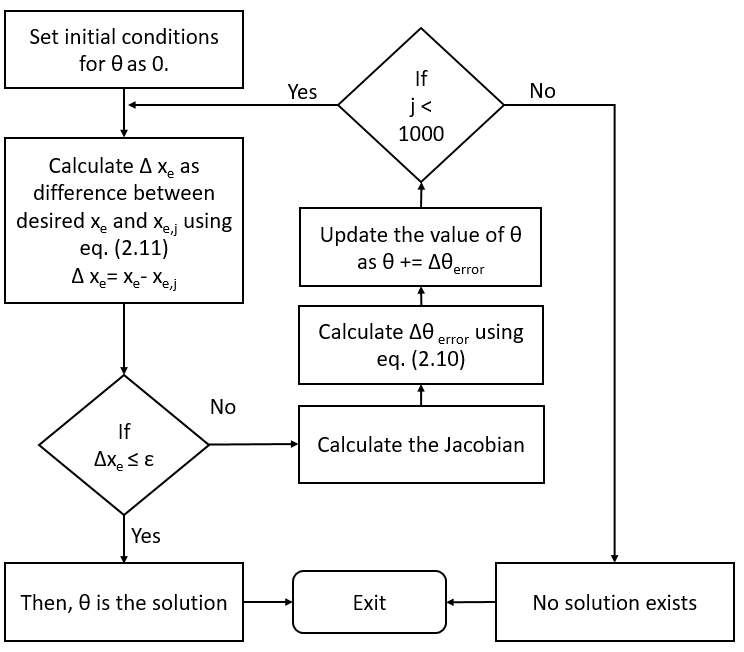
\includegraphics[width=0.6\textwidth]{images/Iteration_2.png}
	\caption{\textit{Flowchart showing the numerical iteration for End-effector Position $\longrightarrow$ Joint Angle Kinematics}}
	\label{iteration-2}
\end{wrapfigure}
\begin{equation}
\label{inv-g3}
\dot{\Theta}=J^{+}\dot{x}_{end}
\end{equation}

However, similar to the situation in subsection \ref{numerical-case-1}, to calculate the Jacobian matrix you need to know the joint angles. It is also a non-linear equation such that the joint angles cannot be separated and hence the equation cannot be calculated analytically. This means that you need to solve this through numerical solution as well. The algorithm used to perform this iteration is shown in Fig. \ref{iteration-2}.

Note that, in the algorithm the differential equation given by eq. (\ref{forward-joint-end}) was modified to numerical form such that in the first step $ x_{end} $ is calculated as:
\begin{equation}
x_{end}= J (\Theta - \Theta_{prev}) + x_{end\_prev} 
\end{equation}

Generally, the end effector position to joint angle inverse kinematic relationship is considered a challenging one. While several methods based on geometry, learning etc. exist to tackle this problem, they are specific to the robotic manipulator that they are being proposed for and often do not apply to manipulators with a different structural design. Still, better methods like the modal method proposed in \cite{RN50} exist for CDHRM. However, for simplicity the numerical method was adopted.

\section{Dynamic Model}
To develop a high performing control for the snake arm, a dynamic model considering the various forces acting on the system is important. To derive the dynamic model, we need to first analyse the forces acting on the system. For any generic robotic manipulator, the dynamic model can be represented as:
\begin{equation}
\label{general-robot-dynamic-eqn}
u = M\left(\Theta\right)\ddot{\Theta} + C(\Theta,\dot{\Theta})\dot{\Theta}+ F_v\dot{\Theta} + g\left(\Theta\right) + J^{T}\left(\Theta\right)F_e
\end{equation}
where, \\
\begin{itemize}
	\renewcommand\labelitemi{--}
	\item $M\left(\Theta\right)$ = Inertia matrix
	\item $C(\Theta,\dot{\Theta})$ = Centrifugal and Coriolis forces
	\item $F_v$ = Coefficient of viscous friction matrix
	\item $g(\Theta)$ = Moment generated by the presence of gravity
	\item $u$ = Actuation torque\footnote{Note that, our system is passive and hence this is 0 in the case of a CDHRM.}
	\item $F_e$ = Force and moment vector exerted by the end-effector on the manipulator. \footnote{This is the terminal condition that is to be defined in the Newton-Euler Recursive algorithm.}
\end{itemize}
A popular method to derive the dynamic model from first principles in this form involves using the Lagrangian method. Another popular method for deriving the dynamic model for robotic manipulators is, Newton-Euler Recursive algorithm. For deriving the dynamic model of CDHRM this method is preferred as it offers higher efficiency \cite{RN30} and does not involve differentiation. 

\subsection{Force Analysis}

\begin{wrapfigure}{t}{0.4\textwidth}
	\centering
%	\vspace{-50pt}
	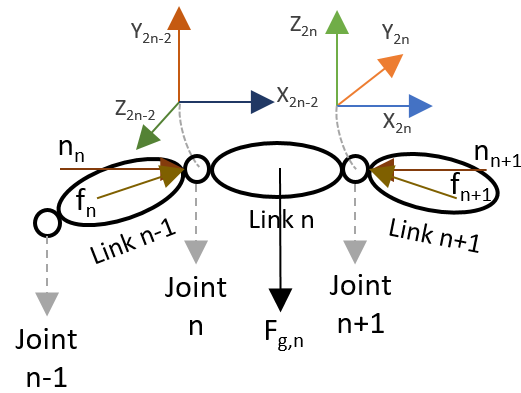
\includegraphics[width=0.4\textwidth]{images/FBD.png}
	\caption{\textit{Free Body diagram showing forces acting on a link (excludes the cable contact and forces).}}
	\vspace{-50pt}
	\label{FBD}
\end{wrapfigure}
One of the steps in the Newton-Euler Recursive algorithm involves using force balance equations acting on a link. Figure \ref{FBD}, shows the free body diagram of the forces acting on the link. Apart from these forces acting on the link there are cable tension forces. Some of the expressions describing these forces are as follows:


\subsubsection{Link Gravitational Force}
Link Gravitational Force is the force acting on the link n due to the presence of gravity. This is given by:
\begin{equation}
^{2n}F_{g,n}=^{2n}R_{0}(-m\hspace{1mm}g_0)
\end{equation}
where,
\begin{itemize}
	\renewcommand\labelitemi{--}
	\item $g$ = acceleration due to gravity given by g = 9.8m/s\textsuperscript{2}
\end{itemize}
In the Newton-Euler Recursive algorithm, the above expression is not explicitly used as gravity as it is considered implicitly in the calculation of linear acceleration as $g_0=[0 \hspace{1mm}0\hspace{1mm}g]^{T}$ acting at the base.
\subsubsection{Link Inertia Force}
The link inertia force can be calculated if the linear acceleration of the centre of mass and inertia are known. 
\begin{equation}
\label{LIF}
^{2n}F_{n}=m\hspace{1mm} ^{2n}\boldsymbol{\dot{v}}_{cn}
\end{equation}
Similarly, if the angular acceleration and velocity are known the link inertia moments can be calculated as:
\begin{equation}
\label{LIM}
^{2n}T_{n} = ^{cn}I_{n}\hspace{1mm} ^{2n}\dot{\omega}_{n} + ^{2n}\omega_{n} \times ^{cn}I_{n}\hspace{1mm} ^{2n}\omega_{n}
\end{equation}
In the above equations:
\begin{itemize}
	\renewcommand\labelitemi{--}
	\item $m$ = mass of a link
	\item $^{cn}I_{n}$ = Inertia Tensor
\end{itemize}
The Inertia tensor $^{cn}I_{n}$ about the frame of reference \{cn\} fixed to the centre of mass of the link can be defined as a diagonal matrix given by the equations for Inertia for a hollow cylinder. This gives:
\begin{equation}
^{cn}I_{n} = 
\begin{bmatrix}
I_{xx} & 0 & 0 \\
0 & I_{yy} & 0 \\
0 & 0 & I_{zz} \\
\end{bmatrix}
\end{equation}
where,
\begin{itemize}
	\renewcommand\labelitemi{--}
	\item $I_{xx}= I_{yy}= \dfrac{m}{4}({r_{outer}^2}+{r_{inner}^2}) + \dfrac{m}{12}(l_{link})^2$
	\item $I_{yy}=\dfrac{m}{2}({r_{outer}^2}+{r_{inner}^2})$
\end{itemize}
\subsubsection{Adjacent Link Interaction Forces}
The interaction between adjacent links subject the link to interaction forces, $f_n$ and $-f_{n+1}$ by the link $n-1$ and link $n+1$ respectively. The link is also subject to a torque $\tau_n$ and $-\tau_{n+1}$ by these adjacent links. These interaction forces has been shown in Fig. \ref{FBD}. These forces and torques can calculated recursively using Newton-Euler Recursive algorithm and this is discussed later on in section \ref{DM-section}.

Note, that the torque described in frame \{2n-1\} has only a x-axis component along $X_{2n-1}$ as the rotation axes of the universal joint, $\zeta_P$ and $\zeta_D$ is consistent with $Z_{2n-1}$ and $Y_{2n-1}$.
\subsubsection{Cable Tension Forces}
When the motor rotates, the cable experiences a tension across it. This can be denoted in terms of its amplitude and direction vector as:
\begin{equation}
\begin{array}{l}
\boldsymbol{F}_{t p, n, k}=F_{t p, n, k} \boldsymbol{e}_{t p, n, k} \\
\boldsymbol{F}_{t d, n, k}=F_{t d, n, k} \boldsymbol{e}_{t d, n, k}
\end{array}
\end{equation}
Given that tension acts along the cable the direction vector $\boldsymbol{e}_{t p, n, k}$/$\boldsymbol{e}_{t d, n, k}$ must be same as the direction vector  $\boldsymbol{e}_{L 1, n, k}$/$\boldsymbol{e}_{L d, n, k}$ representing the direction unit vector of the position vector of the cable. Therefore, 
\begin{equation}
\boldsymbol{e}_{t p, n, k}=\boldsymbol{L}_{p, n, k} /\left\|\boldsymbol{L}_{p, n, k}\right\|
\end{equation}

\begin{equation}
\boldsymbol{e}_{t d, n, k}=\boldsymbol{L}_{d, n, k} /\left\|\boldsymbol{L}_{d, n, k}\right\|
\end{equation}

The global position vector of the cables can be written as:
\begin{equation}
\boldsymbol{L}_{p, n, k}=\left\{\begin{array}{ll}
^{0} A_{2 n}{}^{2 n} \boldsymbol{r}_{p, n, k}-\left[\begin{array}{cccc}
-d & r \cos{\delta_{n,k\textbf{}}} & r \sin{\delta_{n,k}} & 1
\end{array}\right]^{T} & ; n=1 \\
^{0} A_{2 n}{}^{2 n} \boldsymbol{r}_{p, n, k}-^{0} A_{2 n-2}{}^{2 n-2} \boldsymbol{r}_{d, n-1, k} & ; n>1
\end{array}\right.
\end{equation}

\begin{equation}
\boldsymbol{L}_{d, n, k}=^{0} A_{2 n}\left(^{2 n} \boldsymbol{r}_{d, n, k}-^{2 n} \boldsymbol{r}_{p, n, k}\right) \hspace{2mm}; n \geq 1
\end{equation}

where, the homogeneous representation of the hole position can be written as:
\begin{equation}
\begin{aligned}
&^{2 n} \boldsymbol{r}_{p, n, k}=\\
&\left\{\begin{array}{ccccc}
[d-l_{link} & r \sin{\delta_{n, k}} & -r \cos{\delta_{n, k}} & 1]^{T} & (n=\text { odd number }) \\
{\left[d-l_{link}\right.} & r \cos{\delta_{n, k}} & r \sin{\delta_{n, k}} & 1]^{T} & (n=\text { even number })
\end{array}\right.
\end{aligned}
\end{equation}
\begin{equation}
\begin{aligned}
&^{2 n} \boldsymbol{r}_{d, n, k}=\\
&\left\{\begin{array}{ccccc}
[-d & r \sin{\delta_{n, k}} & -r \cos{\delta_{n, k}} & 1]^{T} & (n=\text { odd number }) \\
{\left[-d\right.} & r \cos{\delta_{n, k}} & r \sin{\delta_{n, k}} & 1]^{T} & (n=\text { even number })
\end{array}\right.
\end{aligned}
\end{equation}

Tension in the cable is the force that induces the motion of cables and the change in its length. When the cables move, there is friction between the holes and cables. The frictional force can be related to the force causing the motion which is tension in this case. Therefore, to calculate the value of the magnitude of cable tension forces we recursively use eq. \ref{tension-rec-1} and \ref{tension-rec-2} that are discussed in the part that follows this section. 

\subsubsection{Cable Contact Forces}

As the cables slide in the holes, frictional forces act on the cable. Therefore, the resultant of both the cable tension and the frictional force can be thought of as the contact force of the cable at one hole. Fig. \ref{friction-fig}, depicts the tension forces and also shows that the frictional force, as one would expect, acts opposite to that of the direction of motion\footnote{Note that the direction of motion can also be thought of as the direction of velocity of cables. Therefore, \cite{RN30} discusses computing the sign of the frictional force as the sign of the resultant of velocity of the cable at that point.}. Therefore, frictional forces caused by the sliding motion of the cables can be related to the tension through the following equations:

\begin{align}
&\left\|\boldsymbol{F}_{fr\_p, n, k}\right\|= \left(F_{tp, n, k}+F_{td, n, k}\right)\dfrac{\left(e^{\mu \varphi_{p, n, k}}-1\right)}{\left(e^{\mu\varphi_{p, n, k}}+1\right)} \\
&\varphi_{p, n, k}= \cos ^{-1}\left(e_{tp, n, k} \cdot e_{td, n, k}\right)\\
\label{tension-rec-2}
&e^{\mu \varphi_{p, n, k}}= \dfrac{F_{tp, n, k}}{F_{td, n, k}}\\
&\left\|\boldsymbol{F}_{fr\_d, n, k}\right\|= \left(F_{td, n-1, k}+F_{tp, n, k}\right)\dfrac{\left(e^{\mu \varphi_{d, n-1, k}}-1\right)} {\left(e^{\mu \varphi_{d, n-1, k}}+1\right)}\\
&\varphi_{d, n-1, k}= \cos ^{-1}\left(\boldsymbol{e}_{td, n-1, k} \cdot \boldsymbol{e}_{tp, n, k}\right)\\
\label{tension-rec-1}
&e^{\mu \varphi_{d, n-1, k}}= \dfrac{F_{td, n-1, k}}{F_{tp, n, k}}
\end{align} 

where, $ \mu $ is the coefficient of friction and  $ F_{fr_p,n,k} $ and $ F_{fr_d,n,k} $ acting on the hole $ H_{n,k} $ in the proximal and distal disc respectively.

\begin{wrapfigure}{t}{0.3\textwidth}
	\centering
	\vspace{-30pt}
	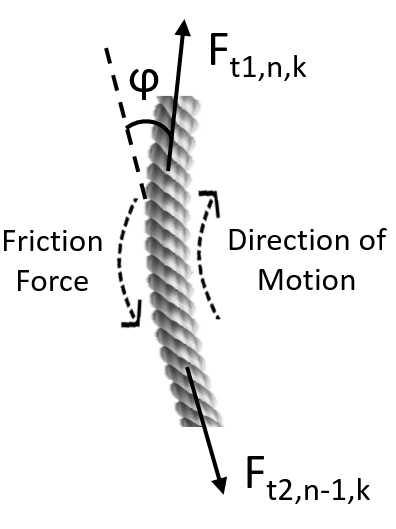
\includegraphics[width=0.3\textwidth, angle=0]{images/Cable forces.png}
	\caption{\textit{ This diagram depicts the direction in which the friction forces act the the forces causing them.}}
%	\vspace{-3cm}
	\label{friction-fig}
\end{wrapfigure}

It has been established that the frictional forces and the normal forces together produce contact forces at the discs. Given this, from above equations that establish the relationship between tension and frictional forces we can derive the contact forces $ F_{c p, n, k} $ and $ F_{c d, n, k} $ acting on the hole $ H_{n,k} $ in the proximal and distal disc respectively, in terms of the cable tension forces acting at that point as: 
\begin{equation}
F_{c p, n, k}=\left\{\begin{array}{cl}
F_{t d, n, k} \boldsymbol{e}_{t d, n, k} & 3 n+1 \leq k \leq 3 N ; n \leq M \\
-F_{t p, n, k} \boldsymbol{e}_{t p, n, k} & \\
-F_{t p, n, k} \boldsymbol{e}_{t p, n, k}, & 3 n-2 \leq k \leq 3 n ; n=M
\end{array}\right.
\end{equation}

\begin{equation}
\begin{aligned}
F_{c d, n-1, k}=& F_{t p, n, k} \boldsymbol{e}_{t p, n, k}-F_{t d, n-1, k} \boldsymbol{e}_{t d, n-1, k} \\
& 3 n+1 \leq k \leq 3 N ; n \leq M
\end{aligned}
\end{equation}
Given this the equivalent contact forces and moments can be denoted as:
\begin{equation}
\label{contact-forces}
^{2 n}F_{e c, n}=\sum_{k=3 n+1}^{3 N} \hspace{0.1pt} ^{2 n}F_{c d, n, k} + \sum^{3 N}_{k=3 n-2}  \hspace{0.1pt} ^{2 n}F_{c p, n, k}
\end{equation}

\begin{equation}
\label{contact-moments}
\begin{aligned}
^{2 n} T_{e c, n}=& \sum_{k=3 n+1}^{3 N}\left(^{2 n}r_{d, n, k} - ^{2 n}P_{c n}\right) \times^{2 n} F_{c d, n, k} \\
&+\sum_{k=3 n-2}^{3 N}\left(^{2 n}r_{p, n, k} - ^{2 n}P_{c n}\right) \times^{2 n} F_{c p, n, k}
\end{aligned}
\end{equation} 

where, $^{2 n} F_{c d, n, k}=^{2 n}R_{0} F_{c d, n, k}$ and $^{2 n}F_{c p, n, k}=^{2 n} R_{0} F_{c p, n, k}$

\subsection{The Inverse Dynamic Model}
\label{DM-section}

\begin{figure}[!tbh]
	\centering
	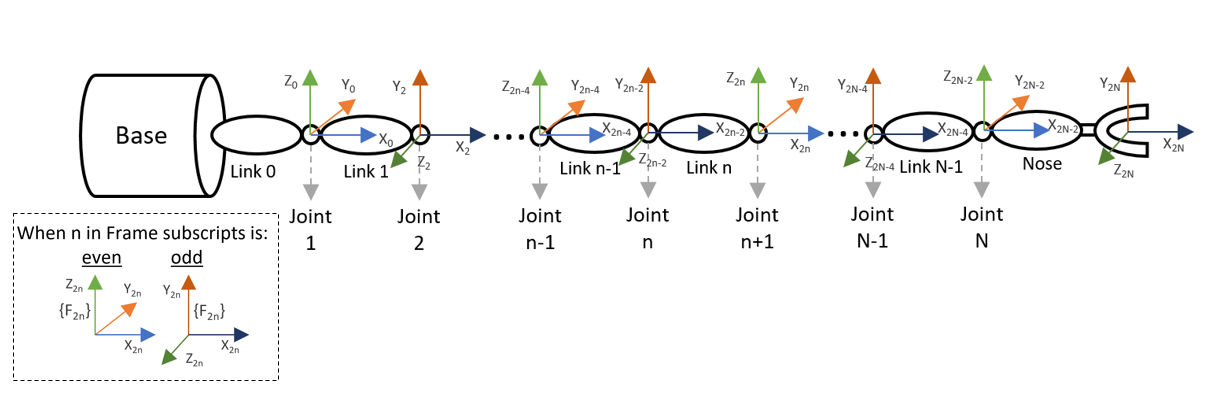
\includegraphics[width=\textwidth]{images/Dynamic Frames.png}
	\caption{\textit{This diagram depicts the frames of reference defined for the derivation of the dynamic model.}}
	\label{dynamic-frames}
\end{figure}
To derive the dynamic model for the CDHRM, Newton-Euler Recursive Algorithm is used here as it offers higher efficiency in comparison to the Lagrange method. Newton-Euler Recursive Algorithm involves two iterations - a Forward Recursion that calculates the velocities and accelerations and a Backward Recursion that calculates the forces and torques. The Newton-Euler method that is described here provides the inverse dynamics relationship. However, the same algorithm can be used to derive back the forward dynamics and this will be discussed in the next chapter. 

\begin{wrapfigure}{t}{0.5\textwidth}
	\centering
	\vspace{-10pt}
	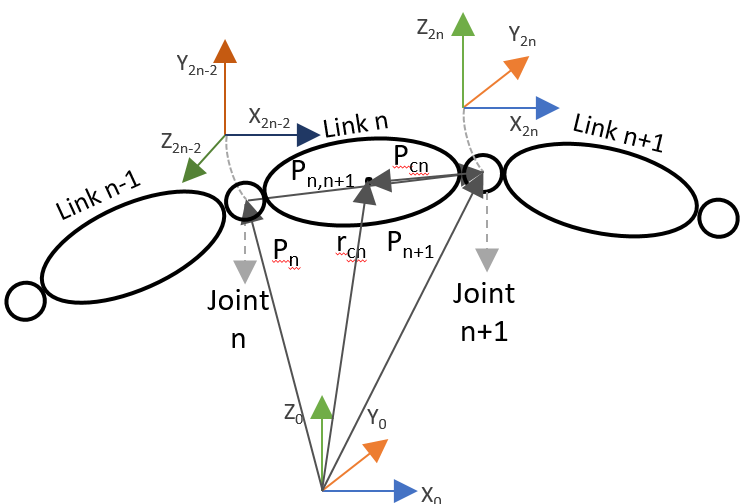
\includegraphics[width=0.55\textwidth]{images/link vector definitions.png}
	\caption{\textit{ This diagram depicts the vectors as per definitions for the Newton-Euler recursive algorithm.}}
	\label{vector-definitions-NER}
	\vspace{-20pt}
\end{wrapfigure}

Before deriving the dynamic model, the reference frames attached to each joint must be established. To keep things simple the reference frame $\{F_{2(n-1)}\}$ is defined at joint n and this corresponds to D-H frames defined in section \ref{forward-jointangle}.The reference frames as defined can be seen in Fig. \ref{dynamic-frames}.


Corresponding to these frames the following position vectors $P_n$, $P_{n,n+1}$ and $P_{cn}$ can be defined for the joints. $P_n$ is the position vector of joint $n$ with respect to base frame. $P_{n,n+1}$ is the position vector from joint $n$ to joint $n+1$. $P_{cn}$ is the position vector of the centroid of link $n$ with respect to $\{F_{2n}\}$. Fig. \ref{vector-definitions-NER} shows these vectors defined for a link $n$.


\subsubsection{Forward Recursion}
The first recursion involves calculation of the angular velocity, angular acceleration and linear acceleration for each link through forward recursion from the base to the end-effector. 

With the initial conditions defined as, $^0\omega_{0}=0\text{ rad/s}$; $^0\dot{\omega}_{0}=0 \text{ rad/s\textsuperscript{2}}$ and $^{0}\dot{v}_{1}=[0\hspace{2mm}0\hspace{2mm}g]^T$ the following expressions can be derived for each link:
\begin{equation}
^{2n}\omega_{n} = ^{2n}R_{2n-2} \hspace{1mm}z_0\hspace{1mm} \dot{\theta}_{2n-1} + ^{2n}R_{2n-1} \hspace{1mm}z_0\hspace{1mm} \dot{\theta}_{2n} + ^{2n}R_{2n-2}\hspace{2.5mm}^{2n-2}\omega_{n-1}
\end{equation}
\vspace{3mm}
\begin{equation}
\begin{split}
^{2n}\dot{\omega}_{n} =& ^{2n}R_{2n-2}\left(^{2n-2}\omega_{n-1}\hspace{1mm} z_0 \hspace{1mm} \dot{\theta}_{2n-1}\right) + ^{2n}R_{2n-2} \hspace{1mm} ^{2n-2}\dot{\omega}_{n-1} + \\ &^{2n}R_{2n-2}\hspace{1mm} z_0 \hspace{1mm} \ddot{\theta}_{2n-1} + ^{2n}R_{2n-1} z_0 \ddot{\theta}_{2n} +\\ 
& ^{2n}R_{2n-2} \times ((z_0 \dot{\theta}_{2n-1}+ ^{2n-2}\omega_{n-1}) \times ^{2n-2}R_{2n-1} z_0 \dot{\theta}_{2n}) 
\end{split}
\end{equation}
\vspace{3mm}
\begin{equation}
^{2n-2}\dot{v}_{n} =
\begin{cases}
^{2n-2}R_{2n-4} \hspace{1mm} ^{2n-4}\dot{v}_{n-1} + ^{2n-2}\dot{\omega}_{n-1} \times ^{2n-2}P_{n-1,n} + \\
^{2n-2}\omega_{n-1} \times (^{2n-2}\omega_{n-1} \times ^{2n-2}P_{n-1,n}) & , n>1\\
\end{cases}
\end{equation}
\vspace{3mm}
\begin{equation}
\begin{split}
^{2n}\dot{v}_{cn} = & ^{2n}\dot{\omega}_{n} \times (^{2n}P_{n,n+1} + ^{2n}R_{2n-2} \hspace{1mm} ^{2n-2}\dot{v}_{n}) + ^{2n}P_{cn} \\
& + ^{2n}\omega_{n} \times (^{2n}\omega_{n} \times (^{2n}P_{n,n+1} + ^{2n}P_{cn})) 
\end{split}
\end{equation}

\subsubsection{Backward Recursion}
The second recursion involves calculating the interaction force and torque acting on each link recursively from the force and moment balance equations. The force and moment balance equations are:
\begin{equation*}
^{2n}F_{n} = ^{2n}f_{n} + ^{2n}F_{ec,n} - ^{2n}R_{2n+2} \hspace{1mm} ^{2n+2}f_{n+1}
\end{equation*}
\begin{equation*}
\begin{aligned}
^{2n}T_{n} = &^{2n}\tau_{n} - ^{2n}R_{2n+2} \hspace{1mm} ^{2n+2}\tau_{n+1} 
- (^{2n}P_{n,n+1}+^{2n}P_{cn}) \times ^{2n}f_{n} \\&- ^{2n}P_{n} \times (^{2n}R_{2n+2}\hspace{1mm}^{2n+2}f_{n+1}) + ^{2n}T_{ec,n}
\end{aligned}
\end{equation*}

With the terminal conditions defined as, $^{2N+2}f_{N+1}=0$ N the following expressions can be derived for each link:
\begin{equation}
^{2n}f_{n} = ^{2n}R_{2n+2} \hspace{1mm} ^{2n+2}f_{n+1} + ^{2n}F_{n} - ^{2n}F_{ec,n}
\end{equation}
\begin{equation}
\label{inverse-dynamic-relationship}
\begin{aligned}
^{2n}\tau_{n} = &^{2n}R_{2n+2} \hspace{1mm} ^{2n+2}\tau_{n+1} + ^{2n}T_{n}
+ (^{2n}P_{n,n+1}+^{2n}P_{cn}) \times ^{2n}f_{n} \\&+ ^{2n}P_{n} \times (^{2n}R_{2n+2}\hspace{1mm}^{2n+2}f_{n+1}) - ^{2n}T_{ec,n}
\end{aligned}
\end{equation}
where,
\begin{itemize}
	\renewcommand\labelitemi{--}
	\item $^{2n}F_{n}$ = Link Inertia force given by eq. (\ref{LIF})
	\item $^{2n}F_{ec,n}$ = Equivalent moment due to contact forces about the centroid given by eq. (\ref{contact-forces})
	\item $^{2n}T_{n}$ = Link Inertia moment given by eq. (\ref{LIM})
	\item $^{2n}T_{ec,n}$ = Equivalent moment due to contact forces about the centroid given by eq. (\ref{contact-moments})
\end{itemize}

From eq. (\ref{inverse-dynamic-relationship}), we now get the dynamic relationship between the driving force (cable tension forces) and the joint angles as\footnote{This is based on the relationship between force transferred to the cable for a certain torque produced by a motor.}:
\begin{equation}
\label{dynamic-to-motor}
\tau_{m,k}=\dfrac{r_{drum}\hspace{1mm}F_{td,0,k}}{\eta}
\end{equation}

Therefore it can be said that eq. (\ref{inverse-dynamic-relationship}) and (\ref{dynamic-to-motor}) together, defines the inverse dynamic relationship for a CDHRM. Using these, we can derive the required torque to be produced by the motor to achieve a required configuration defined by the given joint angles.

\subsection{The Forward Dynamic Model}

In the previous subsection, we used the Newton-Euler Recursive Algorithm to derive the inverse dynamic relationship. Based on eq. (\ref{general-robot-dynamic-eqn}), we can derive the forward dynamic relationship as: 
\begin{equation}
\label{forward-dynamic-relationship}
\ddot{\Theta} = M^{-1}\left(\Theta\right)(u - C(\Theta,\dot{\Theta})\dot{\Theta} - F_v\dot{\Theta} - g\left(\Theta\right)-J^{T}\left(\Theta\right)F_e)
\end{equation}

However, this representation is derived using the Lagrangian method and since the inverse dynamics was discussed based on the Newton-Euler Recursive Algorithm, it would be preferred to use the same to derive forward dynamics using the same as well. \cite{newton-euler-pdf}, proposes a method to do this. It suggest that if used iteratively, the relationship defined by Newton-Euler Recursive Algorithm can be used to derive eq. (\ref{forward-dynamic-relationship}) by setting some of the inputs of the Newton-Euler Recursive Algorithm block to 0 or 1, eliminating terms and isolating the coefficients. The method to do this has been discussed in section \ref{plant-block} in the next chapter.

%%%%%%%%%%%%%%%%%%%%%%%%%%%%%%%%%%%%%%

%%%%%%%%%%% MATHEMATICAL MODELLING %%%%%%%%%%%%%%%%%
\chapter{Implementation and Simulation}

Now that a suitable mathematical model was developed, the second objective of the project was to design a control scheme that would facilitate precise control of the end-effector position. This chapter puts together the different equations discussed in the previous chapter and explains how it was implemented as different blocks on Simulink.  These blocks were then put together as per the proposed control scheme to simulate its behaviour. 

\section{Proposed Control Scheme}

 It is known that the snake-arm robot is indirectly controlled by cables that are attached to the motors at the base of the arm. Based on this knowledge of the inputs and outputs, as a baseline control scheme, the configuration as shown in Fig. \ref{proposed-control-scheme} using the dynamic and kinematic model developed in the previous chapter, was proposed. 
 
 The control objective here is to achieve a very low tracking error (<0.1 mm) for the end-effector position. This mean our reference value is the end-effector position but the value that can be controlled is the angular position of the actuator. Therefore, in the proposed scheme the kinematic model is used to map the reference value from end-effector position to the angular position of the actuator.
 \begin{figure}[H]
 	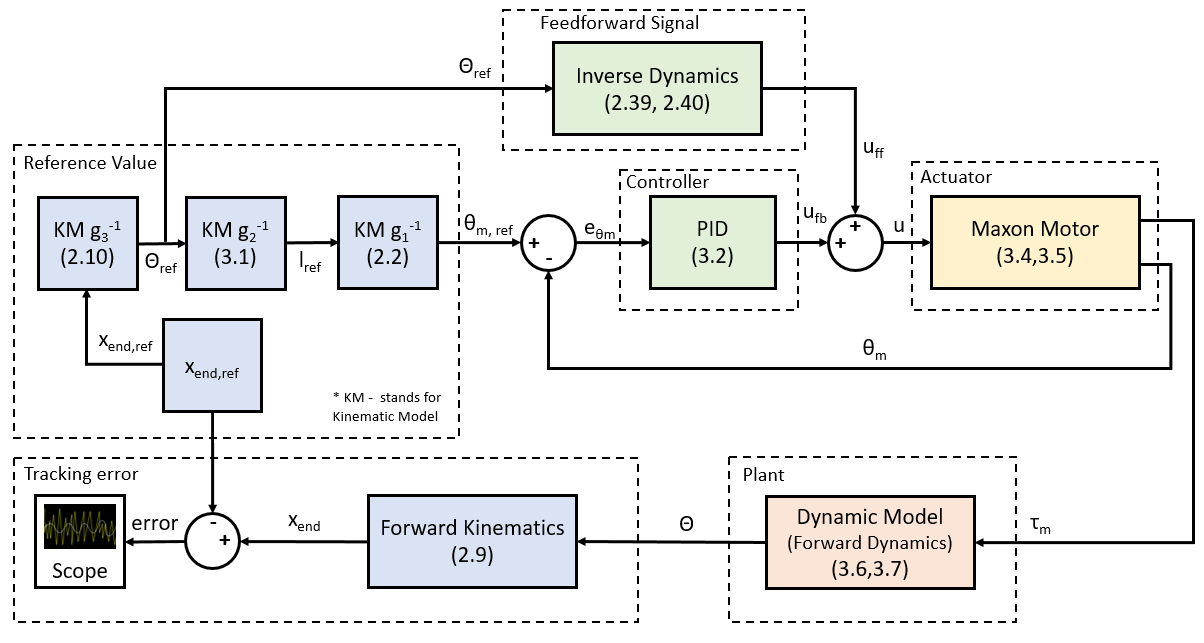
\includegraphics[width=\textwidth]{images/control scheme.png}
 	\caption{The proposed control scheme for the end-effector position control of the CDHRM.}
 	\label{proposed-control-scheme}
 \end{figure}
 The proposed control system design involves a feedforward+feedback control strategy with a PID (Proportional-Integral-Derivative) controller that takes the angular position of the actuator as feedback. This is then summed with a feedforward signal which is derived from the inverse dynamics relationship. The inverse dynamics block is used here to provide an estimate for the required motor torque. The feedforward strategy was introduced as it happens to be a very popular choice for the control of robotic manipulators. However, this decision was also backed by the evidence provided in \cite{RN30} which discusses how using an inverse dynamic block as a feedforward signal improves the performance of the system and reduces the tracking error significantly, based on the results of their experiments on a CDHRM prototype . 

The response of the actuator is then, fed into the dynamic model of the snake-arm and the response from this is mapped back to retrieve the end-effector position to observe the tracking error.


\section{Implementation on Simulink}

\subsection{Dynamic Parameters}
\label{section:dynamic-params}
The equations described in the previous chapter included several dynamic parameters whose values are constant and are usually estimated from the datasheets of the components or the design specifications of the system that is made available. However, for the purpose of this project the idea was to use dynamic parameters from a literature source that describes a similar system. However, all the literature that was identified, associated to dynamic modelling of a CDHRM, performs experiments directly on the actual system and does not discuss a simulation. This meant that the equations for the model as described in this report were compiled from different sources and some were derived. This meant that some of the independent dynamic parameters had to be taken from different sources. Table \ref{dynamic-params}, lists the value used for the simulation.

So, while the values of these parameters were mainly taken from \cite{RN30}, some of the other independent dynamic parameters were assigned based on what was found from different sources. Therefore, these values are possibly not the best estimates of these parameters and could become a reason why the behaviour of the simulated system might deviate from the actual system. A common approach to reducing such parameter estimation errors involves incorporating a regressor term $ Y(\Theta,\dot{\Theta},\ddot{\Theta}) $ in the dynamic model to compensate estimation errors. Another approach involves, modelling the system using Computer-Aided Design (CAD) software to derive some of the physical parameters of the manipulator. To improve the performance further, more sophisticated methods involving learning techniques could also be used. However, all these remain future work and is beyond the scope of this project.

\begin{table}[H]
	\begingroup
	\renewcommand{\arraystretch}{1.5}
	\begin{tabular}{|p{1.8cm}|p{5.4cm}|p{5cm}|}
\hline
\textbf{Notation} & \textbf{Definition} & \textbf{Value} \\
\hline
$N$ & Number of joints & 9 \\
$a$ & Distance between two adjacent universal joints & 140 mm\\
$2d$ & Distance between discs of two adjacent links & 23 mm\\
$m$ & Mass of a link & 0.2 kg\\
$l_{link}$ & Length of the link ($ = a-2d $) & 117 mm\\
$r$ & Radius of the link & 20.5 mm\\
$d_{drum}$ & Diameter of the cable drum & 84 mm\\
$r_{drum}$ & Radius of the cable drum ($ = \dfrac{d_{drum}}{2} $)& 42 mm\\
$p$ & Pitch of the cable drum & 8 mm\\
$k_{trans}$ & Transmission ratio & 0.36\\
$\eta$ & Transmission efficiency & 0.39\\
$J_R$ & Rotor Inertia & 0.864$ \times $ 10\textsuperscript{-7} kg\hspace{1mm}m\textsuperscript{2}\\
$J_L$ & Load Inertia & 0.014 $\times $ 10\textsuperscript{-7} kg\hspace{1mm}m\textsuperscript{2}\\
$k_m$ & Speed-torque Gradient& 0.014 $\times $ 10\textsuperscript{-7} rad s\textsuperscript{-1}N\textsuperscript{-1}m\textsuperscript{-1}\\
$n_0$ & No load Speed& 1007.4 rad s\textsuperscript{-1}\\
$g$ & Acceleration due to gravity & 9.6 m/s\textsuperscript{2} \\
$ \mu $ & Coefficient of friction & 0.17 \\
\hline
\end{tabular}
\endgroup
\caption{Table defining the parameters and its value as used in the simulation.}
\label{dynamic-params}
\end{table}


\subsection{Reference Mapping (Kinematic Model)}

Based on the control objective defined earlier in this chapter, we know that the reference value is the desired end effector position. The unique design of the CDHRM robot implies that joint angles and the end-effector position are not directly controlled by the actuator. This meant that as described by Fig. \ref{reference-mapping}, there are other intermediate spaces between the task space and the control space. So, to map between these spaces a kinematic model had to be developed. From the kinematic relationships defined by eq. (\ref{inv-g3}),(\ref{eq:g1_inv}) and (\ref{third-mapping}), we map the desired end-effector position to the desired amount of angular rotation of the motor.
\begin{figure}[H]
	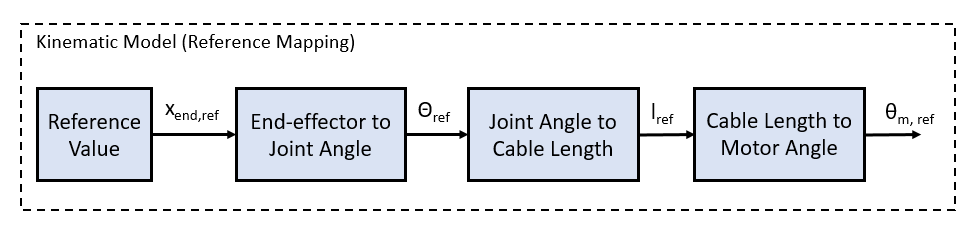
\includegraphics[width=\textwidth]{images/reference-mapping.png}
	\caption{The part of the control scheme that maps the reference alue from the task space to the control space.}
	\label{reference-mapping}
\end{figure}

Note that, eq.(\ref{len_total}) had to be manipulated further to obtain eq. (\ref{third-mapping}) such that the angular position w.r.t initial position\footnote{Initial position here refers to the configuration of the robot when all joint angles are 0.} was calculated. We know, $ L_{0,k} = M\hspace{1mm}l_{link} + n \times (2d) $. Then, the required change in length of the cable can be calculated as $ \Delta L_k = L_k - L_{0,k} $
\begin{equation}
\label{third-mapping}
\Delta L_k = \sum_{j=1}^{M}l_{j,k} - 2nd
\end{equation}


\subsection{Controller Block}

As mentioned earlier, the proposed control scheme involves a feedback + feedforward strategy. 

As can be seen in Fig. \ref{controller-BD}, the feedback signal goes through a PID controller block. So, the output of this block can be described as:
\begin{equation}
u_{fb}=K_P\hspace{1mm}e_{\theta m}(t) + K_I\int_{0}^{t}e_{\theta m}(t')dt' + K_D \hspace{1mm}\dfrac{de_{\theta m}(t)}{dt}
\end{equation}
This signal $u_{fb} $ is then added to the feedforward signal, $ u_{ff} $ which is described in the next subsection.
\begin{figure}[H]
	\centering
	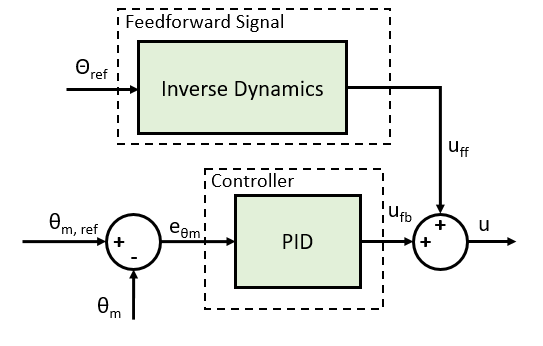
\includegraphics[width=0.7\textwidth]{images/Controller.png}
	\caption{The blocks associated to the controller in the proposed design}
	\label{controller-BD}
\end{figure}

\subsection{Feedforward Block}

The feedforward block uses the inverse dynamics relationship established by eq. (\ref{inverse-dynamic-relationship}) to calculate $ u_{ff} $ . As seen in Fig. \ref{controller-BD}, the feedforward signal block takes the $ \Theta_{ref} $ as the input. However, the equation requires $ \tau_m $ as the input as well and this is unknown. This means that in eq. (\ref{inverse-dynamic-relationship}), there are four unknowns (three of which are values of cable tension that is unknown since $ \tau_m $ is unknown). To simplify this problem and to allow preliminary analysis, $ \tau_m $ was just set to zero as can be seen in the figure in Appendix \ref{appendix d:4}.

\cite{RN30} describes a better and more accurate method to derive the feedforward signal. In the given problem, since $ \tau_m $ is unknown, eq. (\ref{inverse-dynamic-relationship}) will have four unknowns. if three of these are solved by treating the problem as a constrained minimization problem as described below, then the fourth unknown can be calculated (the output) as:
\begin{equation}
\left\{\begin{array}{l}
\text { minimize }: F=\sum_{k=3 n-2}^{3 n} F_{t p, n, k} \\
\text { subject to }:\left\{\begin{array}{l}
^{2 n-1} n_{c, n}=^{2 n-1} R_{2 n}\left(^{2 n} R_{2 n+1}{}^{2 n+1} n_{n+1}^{\prime}\right. \\
-^{2 n} R_{2 n+2}{}^{2 n+2} n_{n+1}+^{2 n} T_{e c, n}^{\prime} \\
\left.+^{2 n} P_{n, n+1} \times \sum_{j=n+1}^{N} 2 n R_{2 j}{}^{2 j} F_{e c, j}\right) \\
R^{\prime 2 n-1} n_{c, n}=R^{\prime 2 n-1} n_{n}^{\prime} \\
F_{t 1, n, k} \geq F_{\min } ;(k=3 n-2, \ldots, 3 n)
\end{array}\right.
\end{array}\right.
\label{minimization}
\end{equation}   

where $^{2 n} \boldsymbol{F}_{c 2, n, k}=^{2 n} \boldsymbol{R}_{0} \boldsymbol{F}_{c 2, n, k},^{2 n} \boldsymbol{F}_{c 1, n, k}=^{2 n} \boldsymbol{R}_{0} \boldsymbol{F}_{c 1, n, k}$ and $ F_{\min } = 40N$. $ F_{\min }$ here is the pretensioning force required to keep cable tense.

After implementing a working version of this block based on the first approach, an attempt was made at implementing this block based on the second approach, however it was unsuccessful and could not be completed.

\subsection{Actuator Block (Maxon Motor)}
\begin{wrapfigure}{r}{0.5\textwidth}
	\centering
	\vspace{-20pt}
	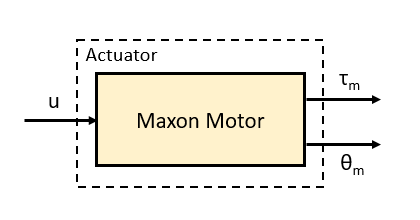
\includegraphics[width=0.6\textwidth]{images/actuator-block-outside.png}
	\caption{Block associated to the actuator in the proposed control scheme}
	\label{maxon-motor}
	\vspace{-30pt}
\end{wrapfigure}
It was identified from online sources that the actuator used here is a maxon motor. Therefore, from its datasheet \cite{maxon-key-information}, it was found that the following model can be used to represent the motor:
\begin{equation}
\ddot{\theta}_{m}=\dfrac{u}{J_L+J_R}
\end{equation}
where,
\begin{itemize}
	\renewcommand\labelitemi{--}
	\item $ J_L $ = Load Inertia
	\item $ J_R $ = Rotor Inertia
\end{itemize}

Based on this equation, the model was implemented on Simulink as shown in Fig. \ref{maxon-motor-BD}. 

\begin{figure}[H]
	\centering
	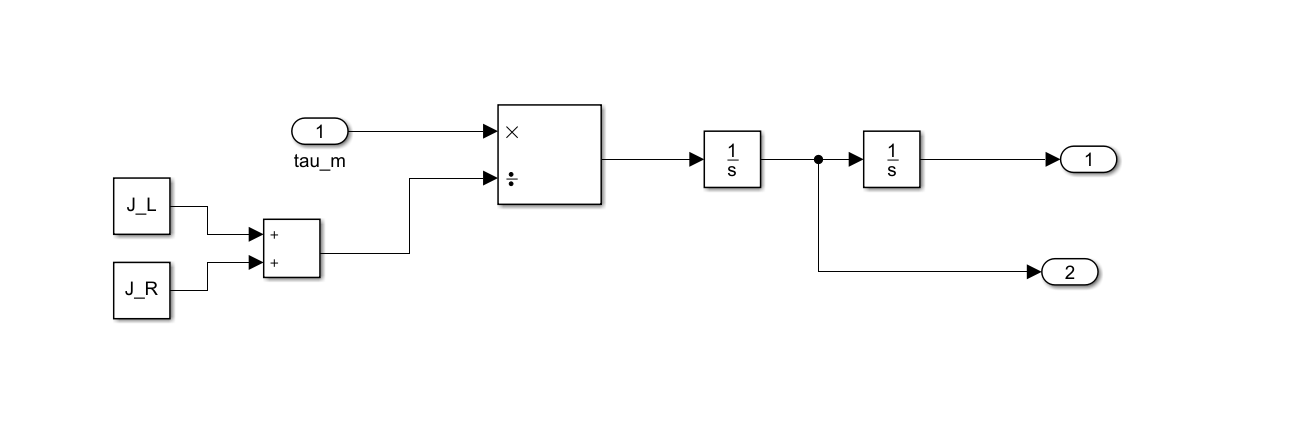
\includegraphics[width=\textwidth]{images/maxon-motor-model.png}
	\caption{Block diagram showing the implementation of the maxon motor model.}
	\label{maxon-motor-BD}

\end{figure}

Further, from the obtained speed the ideal transmitted torque (without loss) is calculated as:
\begin{equation}
\tau_m = n_0 - k_m \hspace{1mm}M
\end{equation}
where,
\begin{itemize}
	\renewcommand\labelitemi{--}
	\item $ n_0 $ = No load speed
	\item $ k_m $ = Speed-torque gradient
\end{itemize}
The value $ \tau_m $ then goes in as input to the robot's dynamic model. Note that, the values for motor characteristics $ n_0 $,$ k_m $,$ J_L $ and $ J_R $ were derived from \cite{maxon-motor-data} for the maxon motor serial number 110063.

\subsection{Plant Block (Dynamic Model)}
\label{plant-block}

\begin{wrapfigure}{h}{0.5\textwidth}
	\centering
	\vspace{-20pt}
	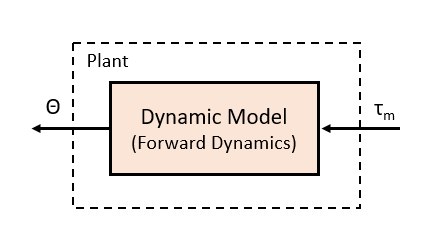
\includegraphics[width=0.6\textwidth]{images/Dynamic Model.png}
	\caption{The block in the control scheme referring to the dynamic model of the system.}
	\label{dynamic-model-implementation}
\end{wrapfigure}
In the previous chapter, we described eq.(\ref{general-robot-dynamic-eqn}) as the general inverse dynamic relationship for the CDHRM and then used the Newton-Euler Recursive algorithm to derive eq. (\ref{inverse-dynamic-relationship}) which is another equation that represents the same system. Therefore, if we think of the block that implements all the equations associated to Newton-Euler Recursive algorithm as a function given by $ NE(\Theta,\dot{\Theta},\ddot{\Theta}) $ then, we can say that: 
\begin{equation*}
u=NE(\Theta,\dot{\Theta},\ddot{\Theta})=M\left(\Theta\right)\ddot{\Theta} + C(\Theta,\dot{\Theta})\dot{\Theta}+ F_v\dot{\Theta} + g\left(\Theta\right) + J^{T}\left(\Theta\right)F_e
\end{equation*}
From this we can derive that, 
\begin{equation}
\label{NE-other-terms}
NE(\Theta,\dot{\Theta},0)= C(\Theta,\dot{\Theta})\dot{\Theta}+ F_v\dot{\Theta} + g\left(\Theta\right) + J^{T}\left(\Theta\right)F_e \\
\end{equation}
Next, the Mass matrix $ M(\Theta) $ can be derived through n iterations. Each iteration i gives one column $ M_i(\Theta) $ of $ M(\Theta) $ such that, 
\begin{equation}
\label{NE-mass-matrix}
	NE(\Theta,0,e_i)= C(\Theta,\dot{\Theta})\dot{\Theta}+ F_v\dot{\Theta} + g\left(\Theta\right) + J^{T}\left(\Theta\right)F_e.
\end{equation}
where, $ e_i $ is the i\textsuperscript{th} column of the identity matrix $ I_{2N} $.
Note that for eq. (\ref{NE-mass-matrix}) to hold true, values of $ g $ and $ F_e $ must be explicitly set to 0. Also, the viscous friction term $ F_v \dot{\theta} $ in eq. (\ref{general-robot-dynamic-eqn}), was omitted for the simulation here.

The figure below shows the block diagram of the dynamic model as implemented in Simulink.

\begin{figure}[H]
	\centering
	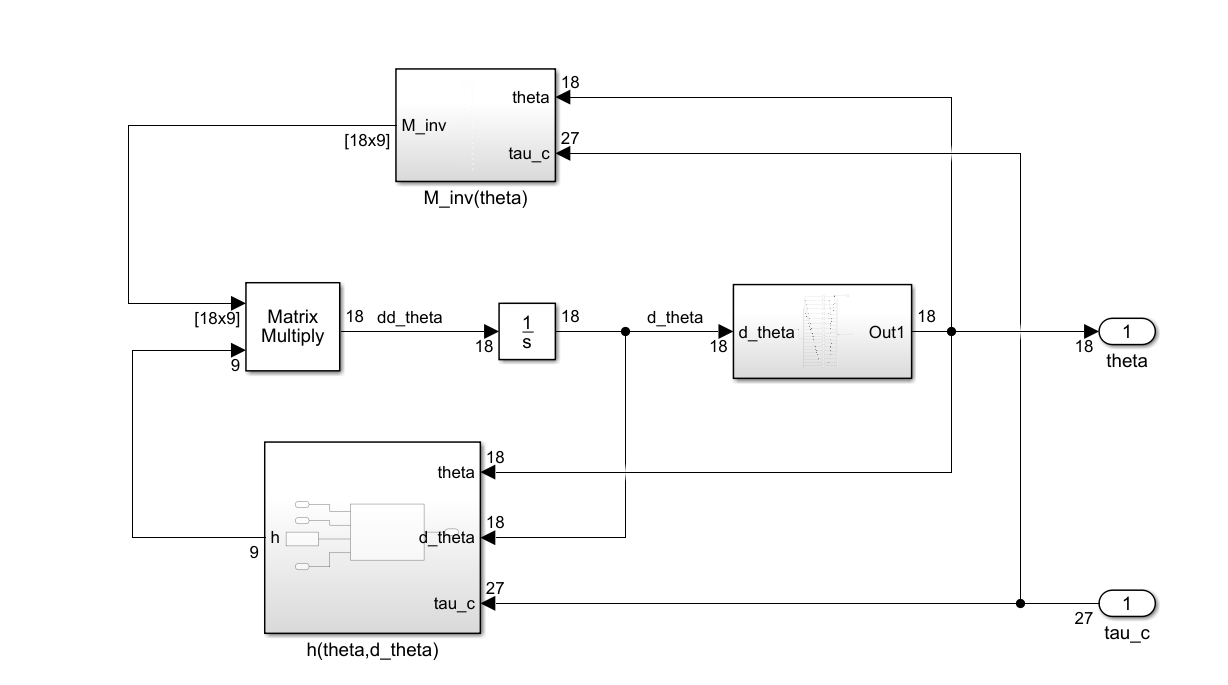
\includegraphics[width=\textwidth]{images/Dynamic-Model_BD.png}
	\caption{Block Digram showing the implementation of the forward dynamics model.}
	\label{dynamic-model-implementation-BD}
\end{figure}
%%%%%%%%%%%%%%%%%%%%%%%%%%%%%%%%%%%%%%

\chapter{Results and Analysis}
\label{result-chapter}
In the previous chapter, the proposed control scheme and the block diagram based on which the Simulink model was implemented was discussed. The blocks that were implemented on Simulink were first cross-validated and then two models in the control scheme were separately tuned to understand their behaviour under the influence of different gains. This chapter discusses the results obtained from these tasks.

\section{Cross-verification of Block Results}
Once the block was implemented and the model was debugged, the next task was to make sure there are no logical errors and that the block behaves as expected. Ideally, one would want to validate the behaviour of the model with the behaviour of the actual system for the same inputs. However, this was beyond the scope of this project and hence the next easiest way to do something similar was to check that if for a known input-output combination, if the output of the inverse relationship block is connected to the input of the forward relationship block for a particular mapping, then these blocks can be considered to have cross validated. Additionally, wherever possible for the same task known values were used.

\subsection{Verifying the Cable Length and Joint Angle Kinematic Model}
To verify the cable length and joint angle mapping of the kinematic model of this system we use the Simulink model as shown below.
\begin{figure}[H]
	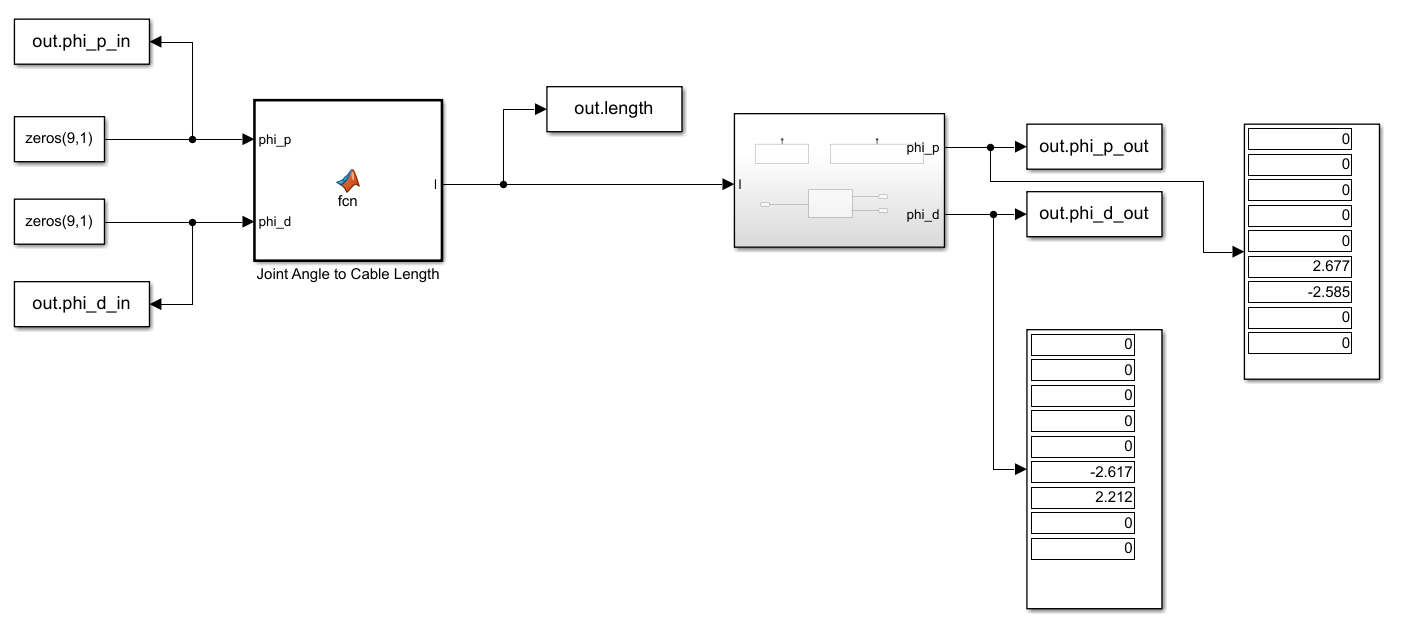
\includegraphics[width=\textwidth]{images/verification-g2.png}
	\caption{The figure shows the Simulink model used to verify the forward and inverse Cable Length and Joint angle kinematic model}
\end{figure}
We know that when, the joint angles are $ 0 $, then the length of cable between 2 links is $ 2d $. This known condition is used to verify the results obtained for the 2 blocks. It can be seen in the above figure that the for an input with all angles set to 0, the output on the other end mostly gives 0. However, there are two exceptions and this might stem from the fact that the given system is hyper-redundant. This means that even for the same change in cable length the robot may be in a different pose. However, it must be noted that on checking the values saved in \texttt{out.length}, this was observed to be $ 2d $ as expected.

\subsection{Verifying the End-effector Position and Joint Angle Kinematic Model}
To verify the end-effector position and joint angle mapping of the kinematic model of this system we use the Simulink model as shown below.
\begin{figure}[H]
	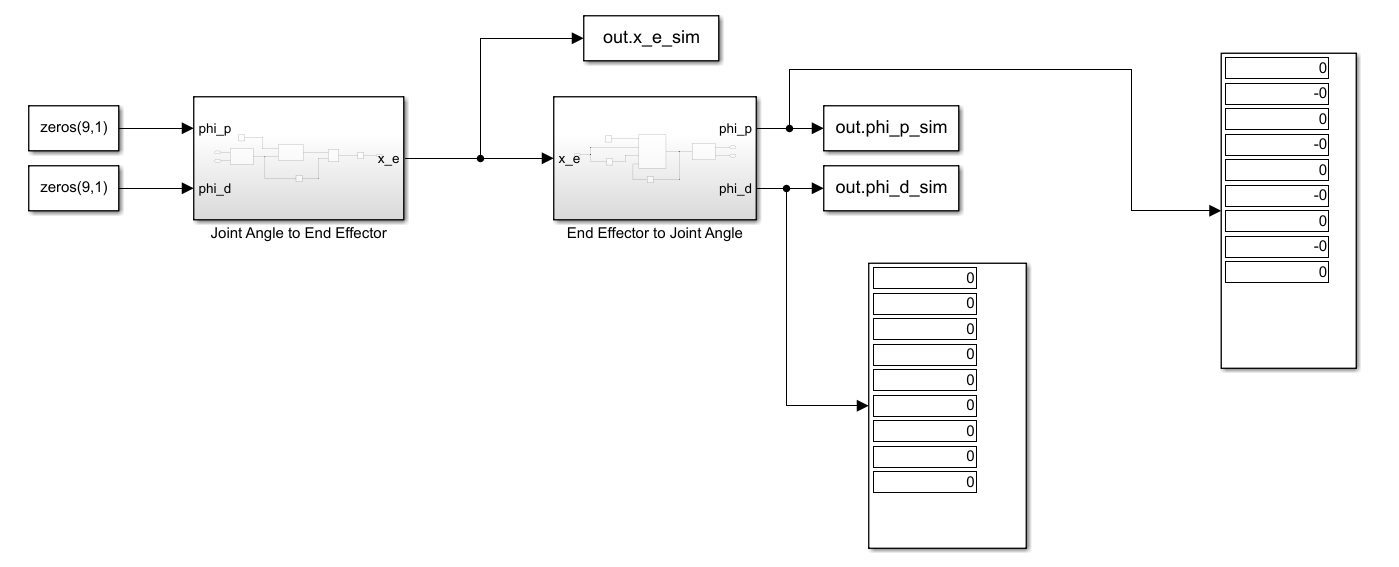
\includegraphics[width=\textwidth]{images/verification-g1.png}
	\caption{The figure shows the Simulink model used to verify the forward and inverse end-effector position and Joint angle kinematic model}
\end{figure}

Unlike in the previous section, here we do not have a know initial condition. However, it can be seen from the results obtained for this setup that the results at the input and the output are the same as desired. This should assure that the blocks perform as expected. 

\subsection{Verifying the Inverse Dynamics Block}

The inverse dynamic relationships obtained from the Newton-Euler Recursive Algorithm was implemented in the block named \texttt{Newton-Euler Inverse Dynamics Block}, shown in the Fig. \ref{ff-sim} below. To debug the block and observe the value at the output end of the Newton-Euler Recursive algorithm the model setup depicted by Fig.\ref{ff-sim} was implemented. 
\begin{figure}[H]
	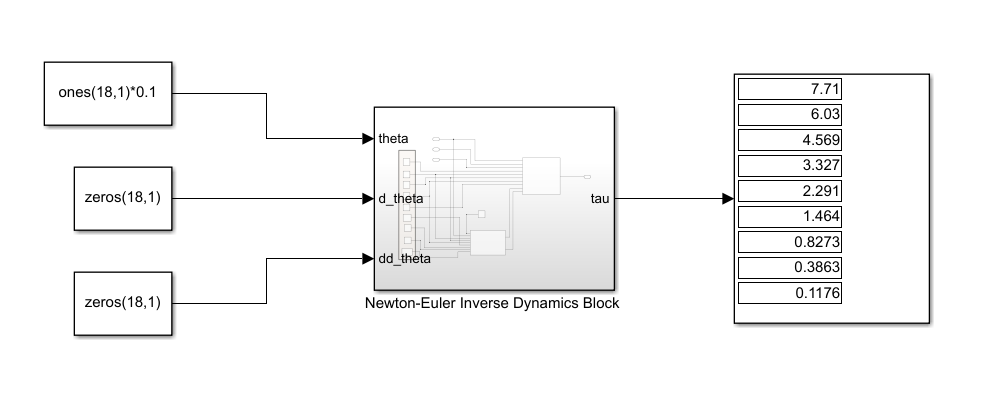
\includegraphics[width=\textwidth]{images/feedforward-block.png}
	\caption{The Simulink model used to verifying the results obtained fro the Newton-Euler Inverse Dynamics Block.}
	\label{ff-sim}
\end{figure}
Additionally, since the same block was attempted to be used as the feedforward signal. This model was used to test the output received when the input \texttt{tau\_c} is made 0 to ensure the outputs are feasible torque values that can be then used as the feedforward signal. When the \texttt{tau\_c} values are mapped to the respective cable tension forces then it was found that they meet the constraints specified by eq. (\ref{minimization}) and hence it was concluded that this is could be a suitable choice as a feedforward signal as well.

\section{Tuning the Controller with the Actuator Model}
In the proposed control scheme, the actuator block includes the dynamic model of the maxon motors. In the actual system, the actuator is what can be directly controlled and so in the proposed scheme the signal fed into the PID controller is the feedback of the angular position of the motor. If we isolate just the actuator with the feedback loop and controller from the control scheme, then we get the model as shown in Fig. \ref{motor-tuning}. 

\begin{figure}[H]
	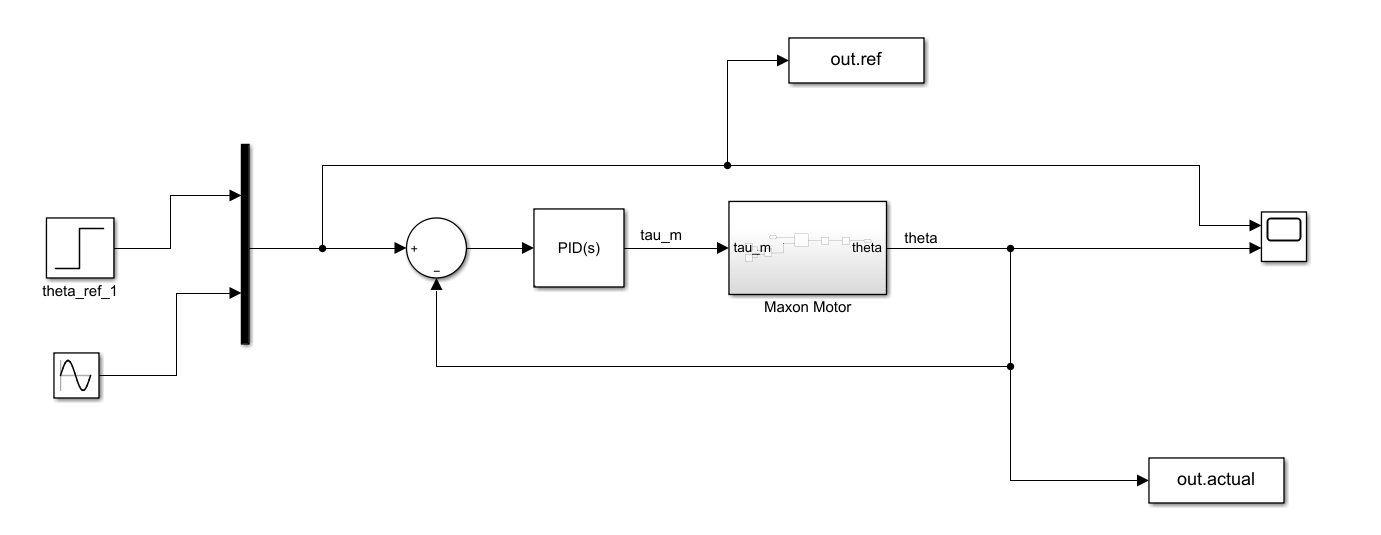
\includegraphics[width=\textwidth]{images/Motor-tuning.png}
	\caption{The Simulink model used for tuning the dynamic model of the motor.}
	\label{motor-tuning}
\end{figure}

The main motivation behind attempting to tune the controller for the  actuator model separately is the fact that the gains obtained from this can be used as the starting point when the controller for the whole system needs to be manually tuned. 

On tuning the PID controller with the dynamic model of the maxon motor, with a step input, a satisfactory response (with a very tiny overshoot at the beginning) as shown in Fig. \ref{step-response} was observed when gain values were set as: $K_P=0.92; K_I=33;K_D=0.005;$.

\begin{figure}[H]
	\begin{subfigure}{.5\textwidth}
		\centering
		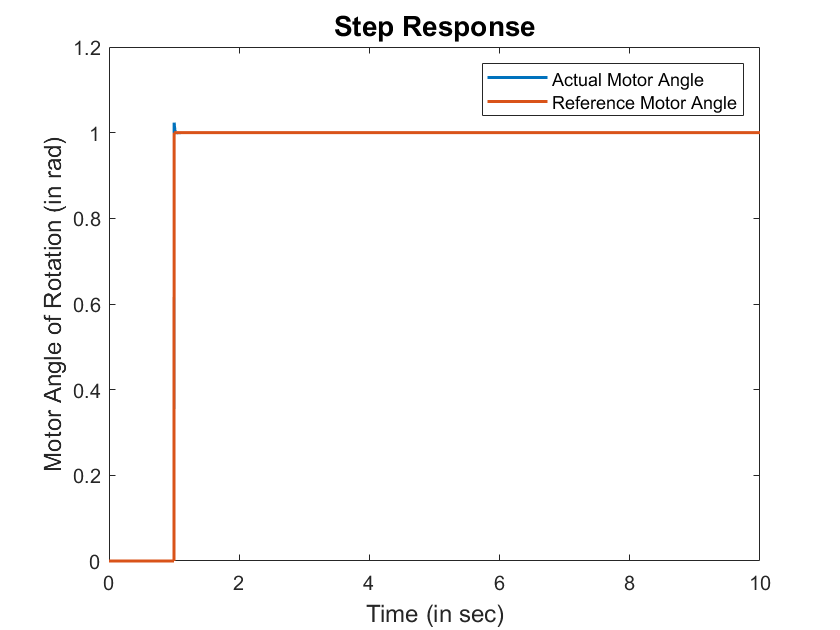
\includegraphics[width=\linewidth]{images/step-response.png}  
		\caption{Reference: Step Signal}
		\label{step-response}
	\end{subfigure}
	\begin{subfigure}{.5\textwidth}
		\centering
		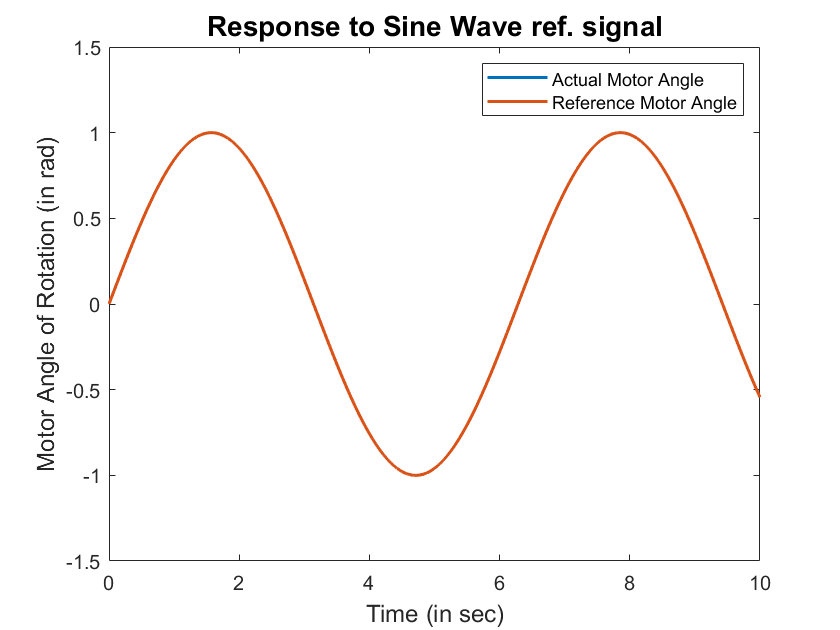
\includegraphics[width=\linewidth]{images/sin-response.png}  
		\caption{Reference: Sinusoidal Signal}
		\label{sin-repsonse}
	\end{subfigure}
	\caption{Response of the tuned motor block to a reference signal}
	\label{response-motor}
\end{figure}

Now that a satisfactory step response was obtained, to ensure that the controller works well for any input, the input was changed to a sinusoidal wave and the response was observed. Fig. \ref{sin-repsonse} shows the response obtained and confirms that the reference value is being tracked well.


\section{Tuning the controller with the Forward Dynamic Block}

After the forward dynamic block was made, to simply test the functionality of the block the model shown in the figure below was implemented. This model isolates the dynamic model block from the other complicated blocks in the proposed control scheme which means that its response to a simple feedback loop configuration can be studied to further understand the behaviour of the system. Note that, here the input reference is a $ 3N\times1 $ vector and the number of outputs is $ 2N\times1 $. Therefore, the feedback is adjusted to match the dimensions of the vector. This is because every 2 joints in between 2 links in the snake-arm are controlled by 3 cables each.

\begin{figure}[H]
	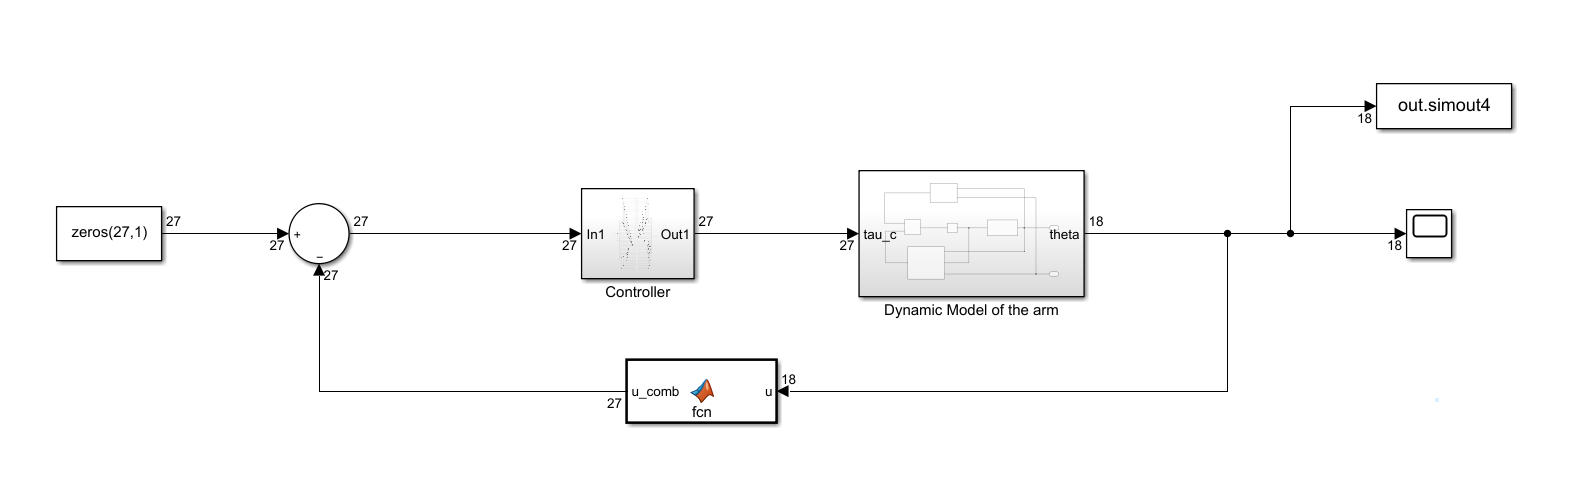
\includegraphics[width=\textwidth]{images/testing-dynamic-model.png}
	\caption{The simplified Simulink model used for tuning the controller with the dynamic model.}
\end{figure}

On trying to run the model, the first couple of attempts failed mid-way through the simulation suggesting unstable behaviour as shown in the Fig. \ref{unstable-responses}. This was mainly because the control gains were not tuned yet. 
\begin{figure}[H]
	\begin{subfigure}{.5\textwidth}
		\centering
		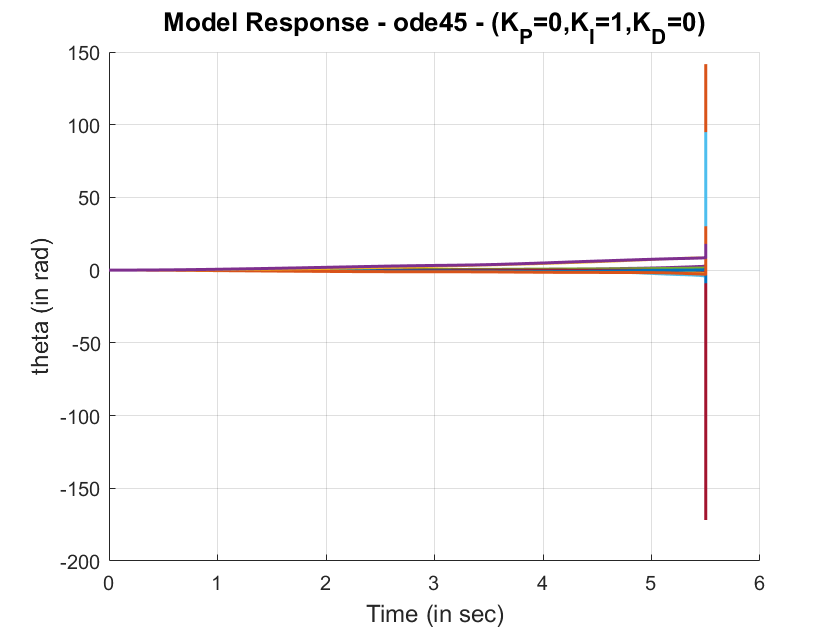
\includegraphics[width=\linewidth]{images/ode45-unstable.png}  
		\caption{Solver: ode45 ; K\textsubscript{P}=0,K\textsubscript{I}=1,K\textsubscript{D}=0}
	\end{subfigure}
	\begin{subfigure}{.5\textwidth}
		\centering
		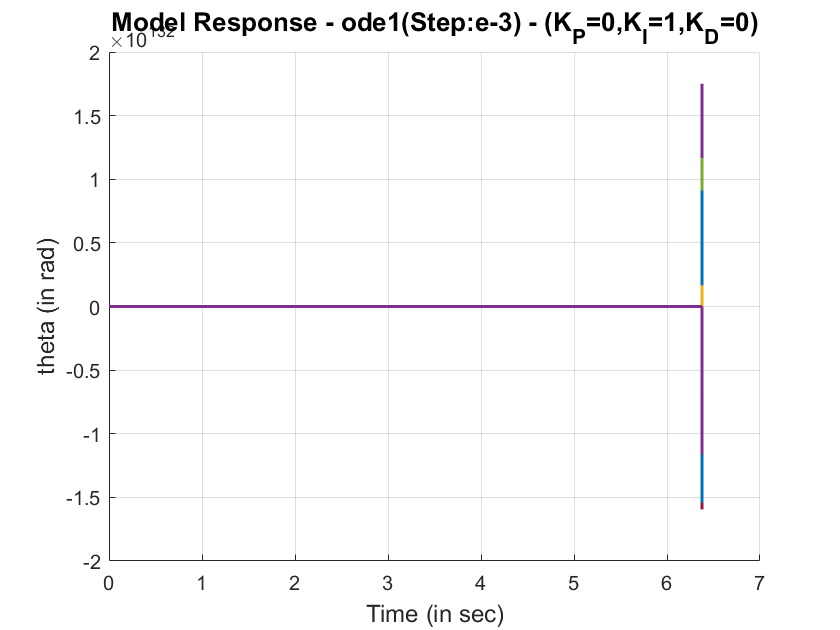
\includegraphics[width=\linewidth]{images/ode1-unstable.png}  
		\caption{Solver: ode1 (Step size=10\textsuperscript{-3}) ; K\textsubscript{P}=0,K\textsubscript{I}=1,K\textsubscript{D}=0}
	\end{subfigure}
	\caption{Unstable responses from the first attempts}
	\label{unstable-responses}
\end{figure}

An attempt was then made to tune the PID controller keeping the same solver, ode1 (Step size=10\textsuperscript{-3}). The simulation time was set to 10s and an attempt was made at manually tuning the gains of the controller. Some of the best results obtained from this attempt, for different gain values, has been shown in Fig. \ref{lumped-responses}. It can be seen here that $ K_P=100;K_I=0;K_D=50 $ shows a smaller peak from among the three. However, since it was unstable, it could not be considered a suitable combination of gains either.

Note that at this stage, only a single PID controller was used for all the 27 inputs. This meant that the attempt at controlling the snake-arm was being made with the assumption that all the joints can be controlled by the same gain value.  

So to make tuning more efficient, each input was assigned a separate controller. This meant that each controller had to be specifically tuned for the joint it was controlling. These were then manually tuned. When trying to control link 1, the best result obtained from among the different gain values that were tried was for: $ K_P=10;K_I=0;K_D=10 $. Similar, tuning was to be done for the other joints, however due to time constraints tuning of all the links could not be completed on time.

However, from the response with the gain values of the tuned controller associated to link 1, the following experiments were done and the observations made are discussed in the following subsections.

\begin{figure}[H]
	\begin{subfigure}{\textwidth}
		\centering
		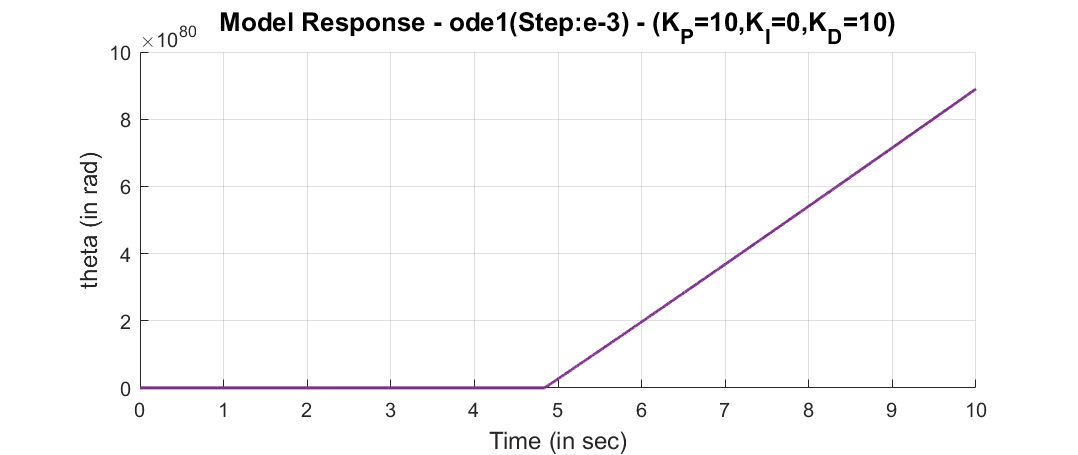
\includegraphics[width=\linewidth]{images/ode1-comp-10-0-10.png}  
		\caption{Solver:ode1 (Step size=10\textsuperscript{-3})  ; K\textsubscript{P}=0,K\textsubscript{I}=1,K\textsubscript{D}=0}
	\end{subfigure}
	\begin{subfigure}{\textwidth}
		\centering
		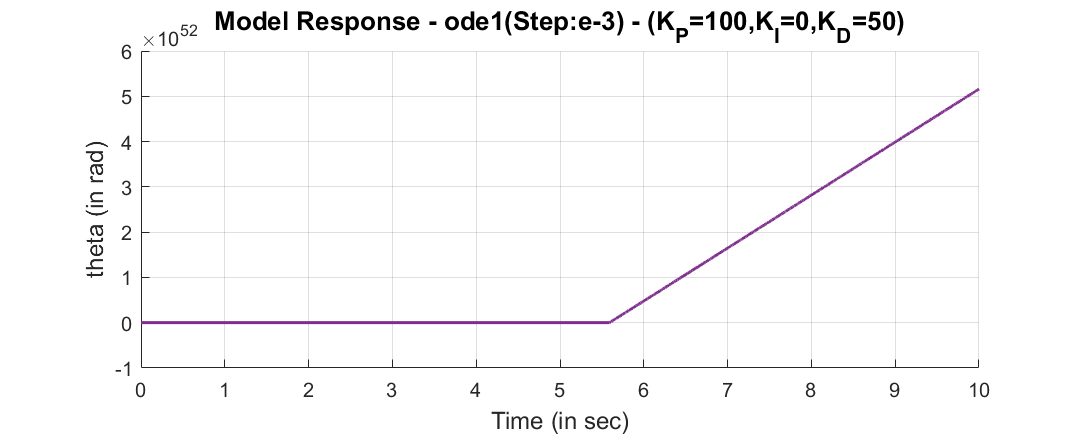
\includegraphics[width=\linewidth]{images/ode1-comp-100-0-50.png}  
		\caption{Solver: ode1 (Step size=10\textsuperscript{-3}) ; K\textsubscript{P}=0,K\textsubscript{I}=1,K\textsubscript{D}=0}
	\end{subfigure}
	\begin{subfigure}{\textwidth}
		\centering
		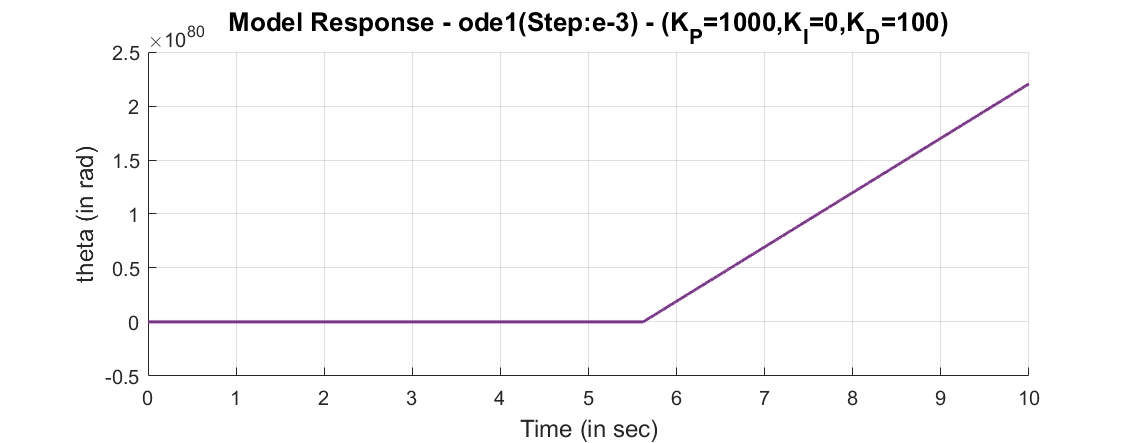
\includegraphics[width=\linewidth]{images/ode1-comp-1000-0-100.png}  
		\caption{Solver: ode1 (Step size=10\textsuperscript{-3}) ; K\textsubscript{P}=0,K\textsubscript{I}=1,K\textsubscript{D}=0}
	\end{subfigure}
	\caption{The responses obtained from attempting to tune a single PID controller that is assigned to all inputs for the snake-arm.}
	\label{lumped-responses}
\end{figure}



\subsubsection{Comparing the use of one controller against three controllers for controlling a link}

It is known that the 2 joints between adjacent links are controlled by 3 cables and this raised the question of whether tuning one controller would be enough to control a joint. So, a comparison was made by controlling the same joint with 1 controller and then 3 controllers of the same gain at the same time.

Fig. \ref{number-of-controllers} below compares the plots obtained on controlling the first 2 joints and the last 2 joints with the same gain values and with the same solver (ode1; Step size: 10\textsuperscript{-3}).

From these plots, it can be observed that not much of a change was observed between the two cases. However, given that the results from the tuned controller are still not very robust it might not be appropriate to make a conclusion based just on this observation.

\begin{figure}[H]
	\begin{subfigure}{0.5\textwidth}
		\centering
		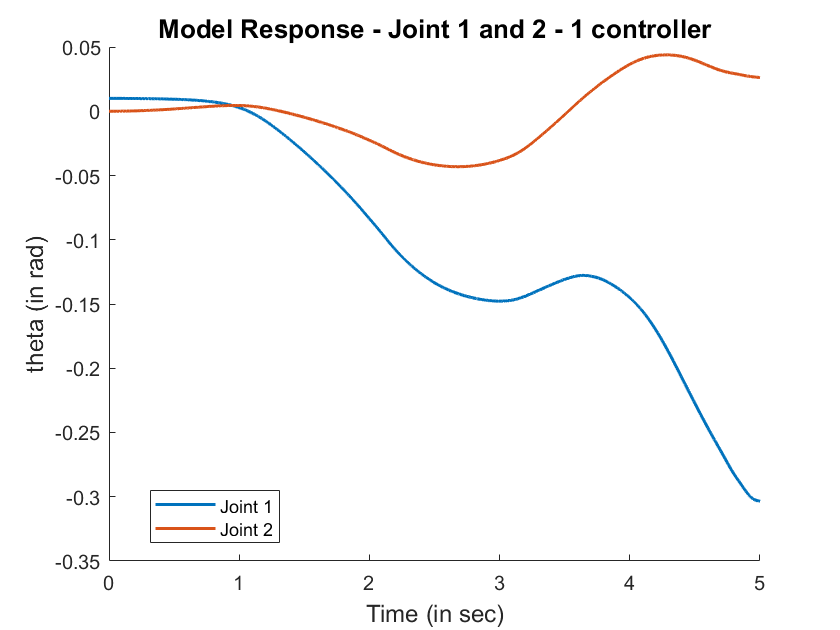
\includegraphics[width=\linewidth]{images/1-controllers-joint1and2.png}  
		\caption{Plot showing the response of joint 1 and 2 on being controlled by only 1 controller}
	\end{subfigure}
	\begin{subfigure}{0.5\textwidth}
		\centering
		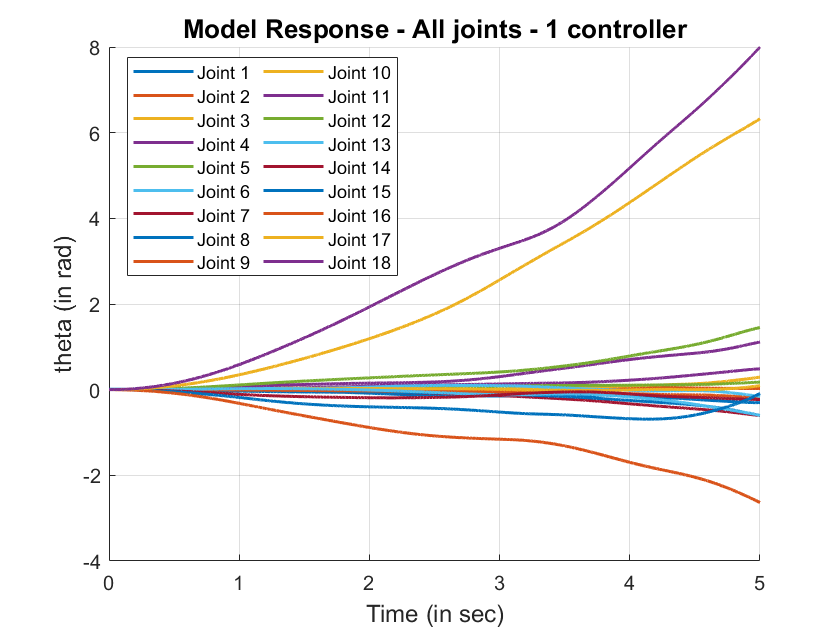
\includegraphics[width=\linewidth]{images/1-controllers-all.png}  
		\caption{Plot showing the response of all other joints when joint 1 and 2 are being controlled by only 1 controller}
	\end{subfigure}
	\begin{subfigure}{0.5\textwidth}
		\centering
		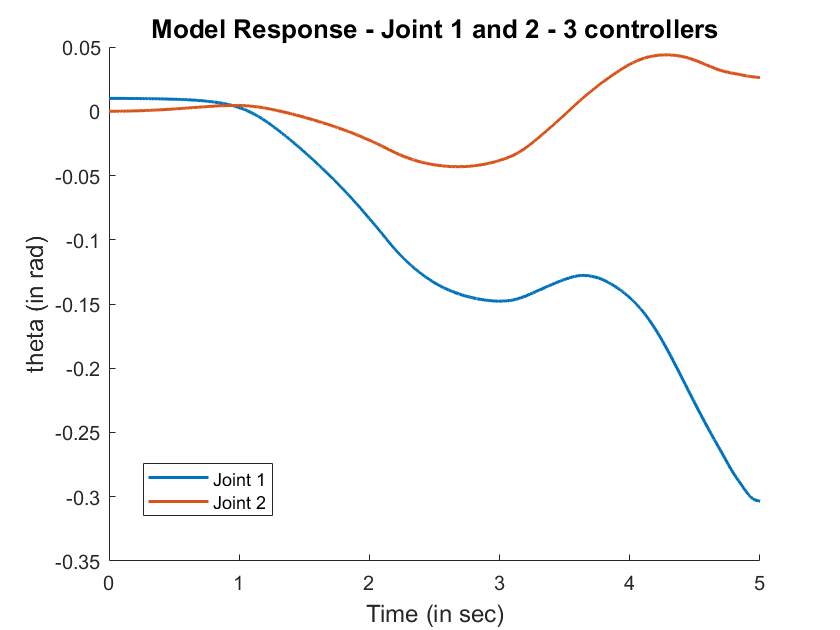
\includegraphics[width=\linewidth]{images/3-controllers-joint1and2.png}  
		\caption{Plot showing the response of joint 1 and 2 on being controlled by 3 controllers at the same time.}
	\end{subfigure}
	\begin{subfigure}{0.5\textwidth}
		\centering
		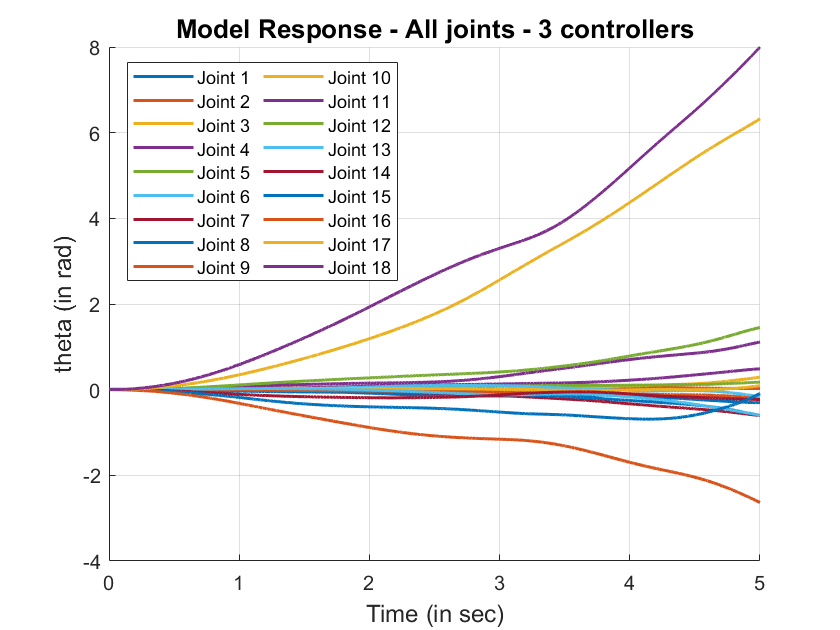
\includegraphics[width=\linewidth]{images/3-controllers-all.png}  
		\caption{Plot showing the response of all other joints when joint 1 and 2 are being controlled by 3 controllers at the same time.}
	\end{subfigure}
	\caption{Comparison of the responses of the dynamic block when the number of controllers controller a joint is increased}
	\label{number-of-controllers}
\end{figure}

\subsubsection{Comparing the plots obtained on controlling the first 2 joints and last 2 joints with the same gain values}

An attempt is made here to try and understand if the same gain values will be effective in controlling different links. For this a comparison is made by controlling the last link with its controller taking the gain values that were tuned specifically for the first link.

Fig. \ref{nth-link} below, compares the plots obtained on controlling the first 2 joints and the last 2 joints with the same gain values and with the same solver (ode1; Step size: 10\textsuperscript{-3}).

From these plots, it can be observed that the response of the first 2 joints are better for the given gain values in comparison to that of the last 2 links. This is a clear indication of the fact that each controller has to be tuned separately for each joint which means that the initial attempt of using a single PID controller was insufficient. As expected, from the plots showing the responses of all joints, it can be clearly seen that depending on which joint is being controlled the joints adjacent to the links being controlled are the most affected while the others don't experience much of a perturbation from the movement of the other links.
\begin{figure}[ht]
	\begin{subfigure}{0.5\textwidth}
		\centering
		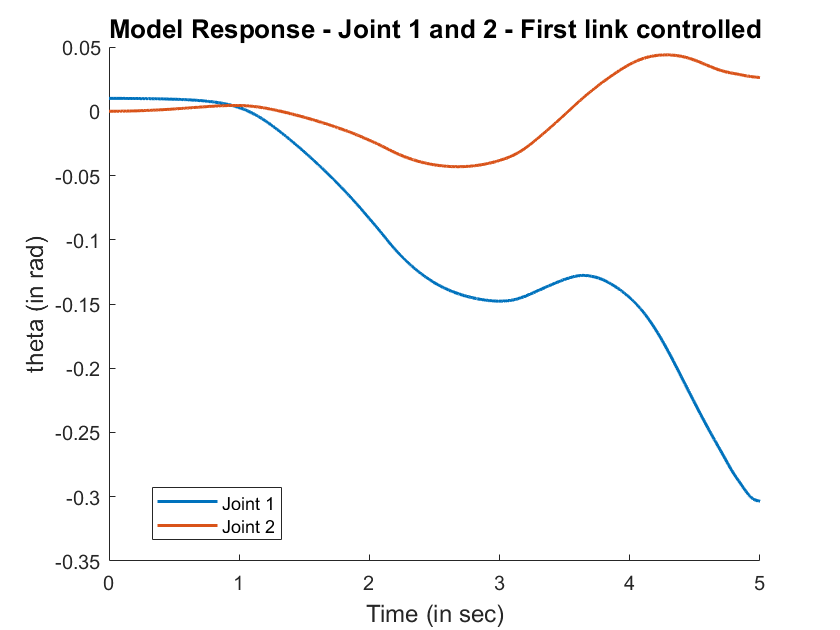
\includegraphics[width=\linewidth]{images/first-2.png}  
		\caption{Plot showing the response for first 2 joints when they are directly controlled}
	\end{subfigure}
	\begin{subfigure}{0.5\textwidth}
		\centering
		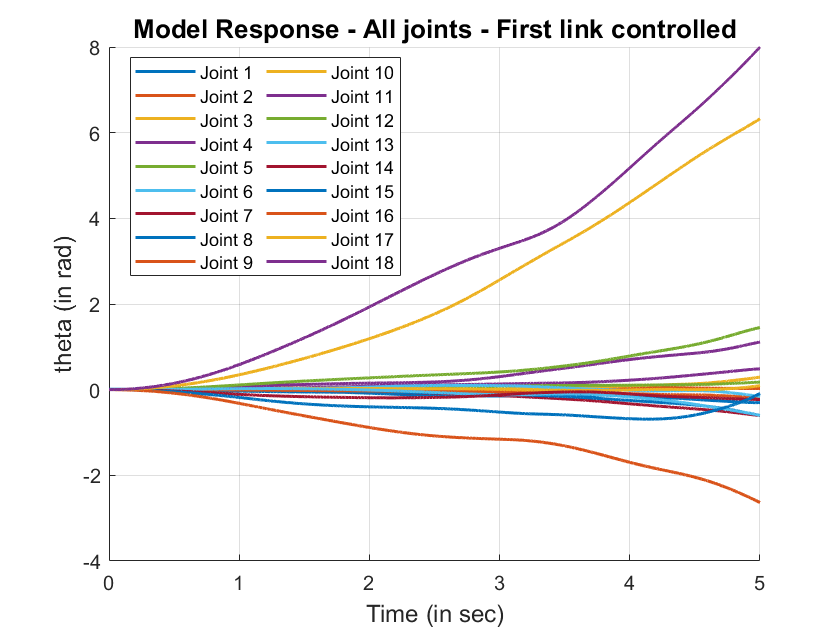
\includegraphics[width=\linewidth]{images/first-all.png}  
		\caption{Plot showing the response for all joints, when only the first 2 joints are controlled}
	\end{subfigure}
	\begin{subfigure}{0.5\textwidth}
	\centering
	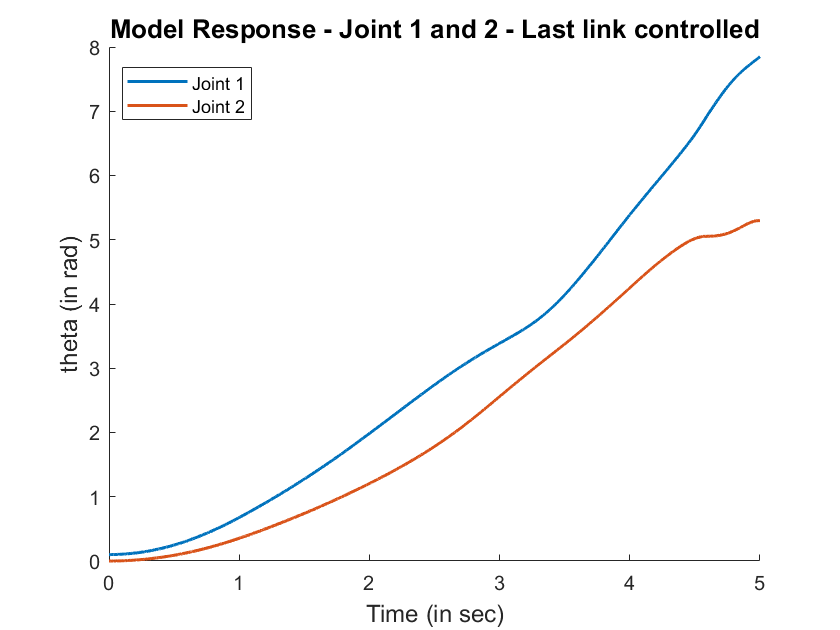
\includegraphics[width=\linewidth]{images/last-2.png}  
	\caption{Plot showing the response for last 2 joints when they are directly controlled}
	\end{subfigure}
	\begin{subfigure}{0.5\textwidth}
	\centering
	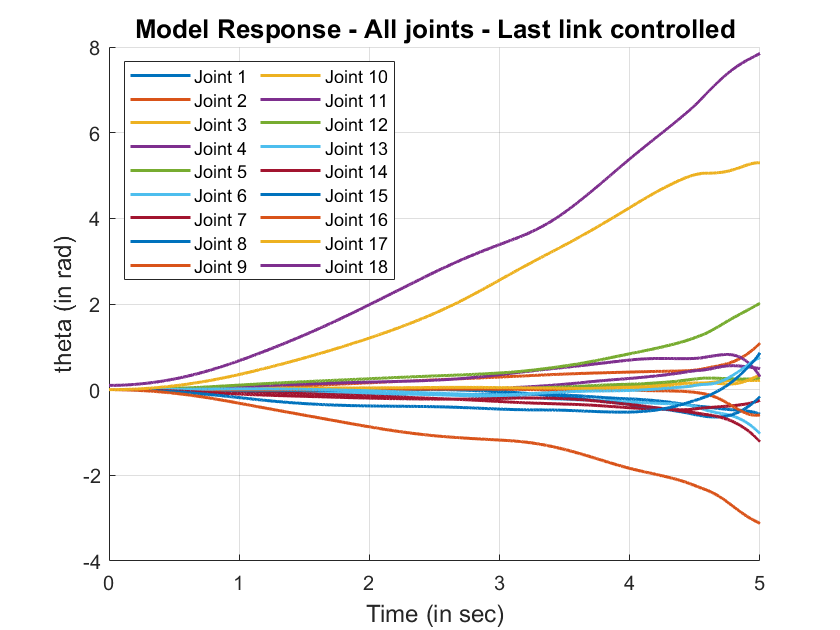
\includegraphics[width=\linewidth]{images/last-all.png}  
	\caption{Plot showing the response for all joints, when only the last 2 joints are controlled}
	\end{subfigure}
	\caption{Comparison of the responses of the dynamic block when only two different links are controlled at at time}
	\label{nth-link}
\end{figure}



\section{Analysis of Robustness}

Since the tuning of the controller could not be completed within the given time constraints, the task associated to evaluating the control scheme's robustness could not be achieved. However, if the controller was tuned the analysis of the robustness of the control scheme would have been done based on two tests.

The first analysis would have been based on the effect of changing load at the nose of the snake-arm. The effect of change in load can be incorporated into the dynamic model by considering the term $ J^TF_e $ in eq.(\ref{general-robot-dynamic-eqn}) into the dynamic model equation. If the Newton-Euler recursive algorithm was to be used instead, $ F_e $ should be set as the terminal condition which has been otherwise set as 0 in the above analysis. Thus in this manner the robustness of the control scheme to changing load could have been analysed by comparing the response in the presence of different $ F_e $ values at the nose of the manipulator.

The second analysis would have been based on the effect of external disturbances. In the Newton-Euler recursive algorithm this would have been incorporated as an additional force term, $ F_ext $ acting at the centroid of the link. Similar to the previous analysis, if the controller would have been tuned, the robustness of the control scheme to changing environments (presence of external disturbances) could have been analysed by comparing the response in the presence of different $ F_ext $ values acting on individual links.


%%%%%%%%%%% CONCLUSIONS %%%%%%%%%%%%%%%%%
\chapter{Conclusions}
% Summary and limitations of what was achieved
This project aimed at developing a dynamic model for a robotic snake-arm manipulator at Here East as an attempt towards contributing to the modelling and control research effort undertaken for this system. The project also aimed at designing a control scheme that would facilitate accurate end-effector position control so that precise trajectory tracking could be achieved. For this, the control system design and the dynamic model was developed, implemented and evaluated using Simulink. 

The previous chapters discussed the derivation of the mathematical model, the proposed baseline control scheme and the preliminary results obtained from the attempt. The individual blocks of the mathematical model were developed, implemented and cross-verified mathematically. However, progess was slow and so only preliminary results for the dynamic model could be achieved as discussed in Chapter \ref{result-chapter}. This meant that only some of the objectives as stated in Chapter 1 could be achieved.

% Why goals werent achieved 
There were several reasons for this. It can be seen in the Gantt Chart in Appendix \ref{appendix:a}, that was submitted along with the proposal that, not much time was allocated for identifying and developing the mathematical model of the system. This was mainly because it was assumed from the work undertaken during summer that the dynamic model would be similar in nature to that of a wheeless-snakebot that moves on the ground. For such a ground-hugging snakebot the mathematical model was derived from first principles of motion and did not involve a lot of background theory. However, the model for this manipulator required a lot more understanding about the theory of dynamic modelling of robotic manipulators in general and the different algorithms/approaches associated to it in order to recognize the equations. This was realised a month into the project and the learning curve cost time, much more than anticipated. The lack of suitable resources discussing the dynamic model and its simulation also contributed to the slower progress in the initial phase. Learning the theory and attempting simpler examples to develop a better understanding of the subject, itself took a month or two of term time.

While the other commitments during term time were also taken into consideration while proposing the objectives, the underestimation of the learning curve meant that project demanded more time than what was initially anticipated. However it can be said that, if the dynamic model and the background theoretical knowledge required to recognise the equations been identified prior to the start of the project during summer, it would have given the head start that was required to be able to achieve all the objectives with the constraints of term time.

In order to simplify the situation, midway through the project an attempt had been made to adopt a simpler approach that involved considering the CDHRM system like just any other general robotic manipulator but with alternate links of length 0 to incorporate the fact that there are two revolute joints between each link. This meant that the standard functions and the general dynamic block provided by the Robotics Toolbox in  MATLAB could be used to develop the control scheme. However as this was attempted, it was realised that for the unique structural design of the CDHRM using the general dynamic block is not a feasible option as this robotic manipulator is a passive system that is indirectly driven by cable tension forces. This meant that to formulate the dynamic response of the system the cable tension forces had to be intrinsically included and this was not an option provided by the function available via the Robotics Toolbox. Hence, this approach was abandoned. 

\section{Future Work}

While this report discusses a suitable mathematical model and proposes a scheme that could be the baseline configuration for the control system of the snake arm, there is more work to be done to be able to achieve the bigger aims of this project. 

Even though the equations of the mathematical model were cross-verified mathematically, the behaviour of the dynamic model is yet to be validated against the behaviour of the actual system. If the dynamic model fails to represent the actual system, then may be an alternate modelling approach could be to use functionalities available within MATLAB like Simscape to use the input and output plant variables recorded from the actual system to develop a dynamic model.

It can be realised that the proposed control scheme also has a lot of room for improvement. For starters, a better control scheme could be something that incorporates feedback from the tracking error of the end-effector position as input to the controller along with the feedback from the angular position of the actuator itself. Another improvement could also be to incorporate force control to regulate the cable tension forces directly, as that is the driving force of the passive robotic arm under consideration that ultimately determines its resulting physical configuration.

Lastly, another aspect about the project that can be explored is the dynamic parameter estimation. Initially, the idea was to use dynamic parameters from one of the literature sources that describes the simulation of a similar system. However, all the literature that was identified, associated to dynamic modelling of a CDHRM, performs experiments directly on the actual system and often did not discuss simulation of the dynamic model. This meant that the equations for the model as described in this report were compiled from different sources. So, while mainly all parameters were defined from \cite{RN30}, some of the dynamic parameters (that were independent) were assigned based on what was found from different sources as a single source covering all parameters could not be identified. Future attempts can possibly rectify this by using the parameters from the actual system. However it is a known issue that even this could result in parameter estimation errors. A common approach to reducing such estimation errors involve incorporating a regressor term like $ Y(\Theta,\dot{\Theta},\ddot{\Theta}) $ in the dynamic model to compensate these errors. This might be something that could be considered given that the estimation of parameters like Inertia tensor tend to introduce errors given the structural design of the manipulator. To improve the performance further, even more sophisticated methods involving learning techniques could be considered.

\vspace{5mm}
To conclude, while this report proposes a suitable mathematical model that represents the actual system under consideration, the proposed control scheme needs improvement. From the discussion on preliminary results, it is evident that more work needs to be done in order to obtain satisfactory results. More control schemes need to be designed and tested in the future until a suitable one that meets the control objective is developed.


%%%%%%%%%%%%%%%%%%%%%%%%%%%%%%%%%%%%%%

%%%%%%%%%%% APPENDIX %%%%%%%%%%%%%%%%%
\begin{appendices}
	%%%%%%%%%%%%%%%%%
	\chapter{Project Gantt Chart {\normalsize (as submitted with proposal)}}
	\label{appendix:a}
	This appendix discusses the Project work plan and Gantt Chart as submitted in the project proposal.
	The project will mainly have four phases - \textit{Preparatory phase, Simulation and Modelling, Testing and Improving results} and \textit{Analysis and Compilation of Results}
	\begin{itemize}
		\item \textbf{Preparatory Phase:} The first month and a half will involve preparatory phase during which through literature review several suitable mathematical models will be identified and the model that best represents the physical snake-arm will be implemented. During this phase the control objectives of the snake arm will also be clearly investigated and will be defined mathematically.
		Work undertaken over summer proved that the approach of mimicking a biological snakebot to improve reach and span of the robot will not be suitable, as controlling such a snakebot poses a lot of challenges. Even though extensive research over the years have led to improved results, the level of accuracy of the tracking of the controlled variable is lower than what is required for a task like air wing inspection. The risk of a snake-arm making contact with the structures due to incorrect path following can be very unsuitable for this scenario. Also, given that the OC Robotics snake-arm is more like a tethered continuum robot moving in free space, the viscous friction model adopted by most authors to describe the dynamic model of a wheel-less ground-hugging robot snakebot won’t be suitable. Therefore, the initial approach when modelling the snake-arm the concept of continuum robots may be used the most.
		\item \textbf{Simulation and Modelling:} The next phase of the project will then involve implementing the mathematical model, simulating the control system on Simulink and obtaining the initial results. The tracking error of the parameters (specially speed, position and orientation) will be analysed and efforts will be made to improve these results. It is expected that at this stage, an iterative testing method would be adopted to improve the model until desired tracking accuracy is obtained.
		\item \textbf{Testing and Improving Results:} From the start of the second phase to the end of the project, results will be improved and tested iteratively until desired results are achieved. Although this has been specified as a separate phase it represents the steps that are part of the second and the last phase. 
		\item \textbf{Analysis and Compilation of Results:} Once satisfactory results are obtained; the final phase of the project will focus on testing the robustness of the system in varied conditions. It is expected that the payload attached to the head will change depending on the optical metrology technique for which it is being used. Further, it might be performing measurements in environments where external disturbances are no longer negligible. So, for these scenarios, tests will be performed to analyse the robustness of the system to these disturbances.
		Results obtained will be reported systematically and periodically through progress reports that are roughly due once in every three weeks since the start of the project.
	\end{itemize}
	
	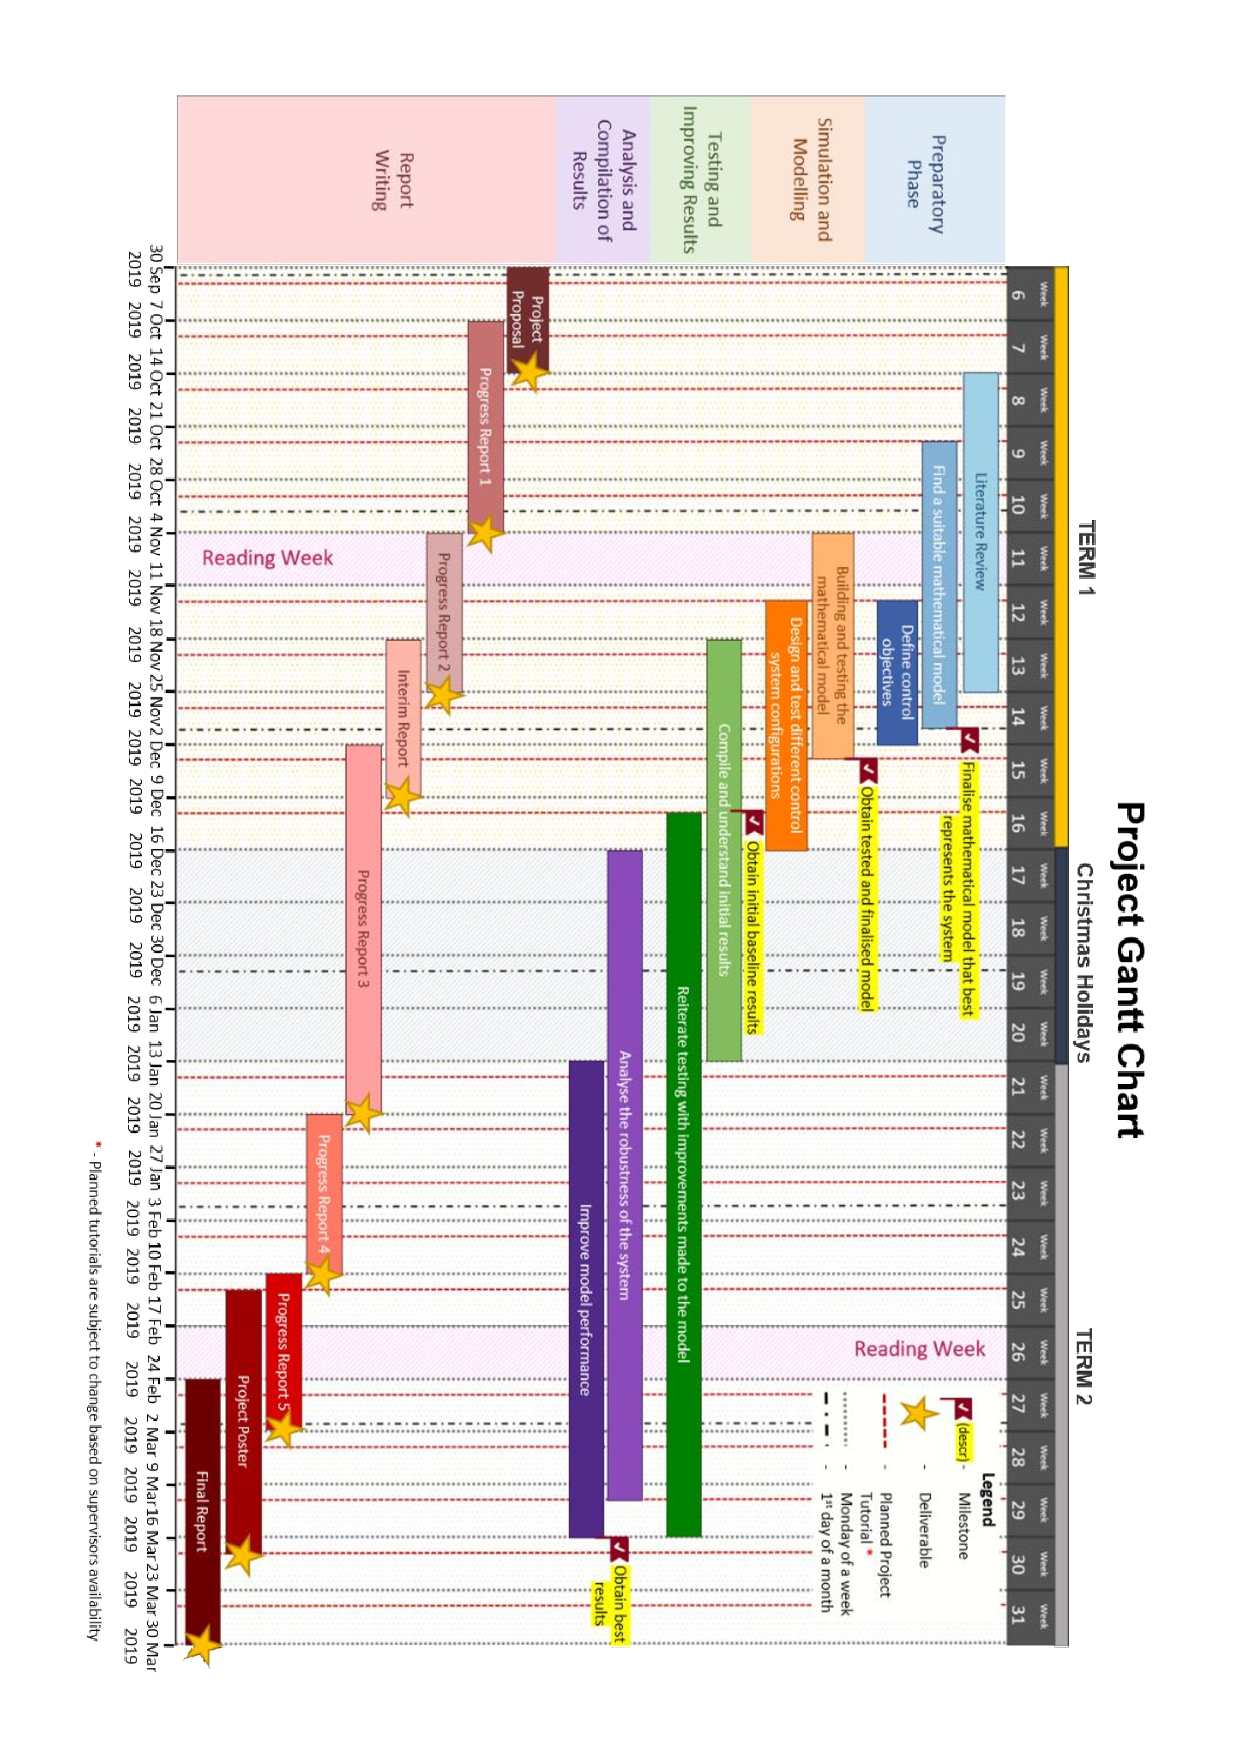
\includepdf[page=-]{files/Gantt Chart}

	%%%%%%%%%%%%%%%%%
	\chapter{List of Notations}
	\label{appendix:notations}
	\begin{center}
		\begingroup
		\renewcommand{\arraystretch}{1.5}
		\begin{longtable}{|c|p{12cm}|}
			\hline
			\textbf{Notation} & \textbf{Definition}  \\ 
			\hline
			\multicolumn{2}{|c|}{\textbf{Subscripts}} \\
			\hline
			$N$ & Number of joints (N=9) \\
			$n$ & \makecell[l]{Subscript that can take values from the set \\ $n=\{1,2,3,\ldots,N\}$ (used for joints)} \\
			$k$ & \makecell[l]{Subscript that can take values from the set \\ $k=\{1,2,3,\ldots,3N\}$ (used for motors, cables)} \\
			$i$ & \makecell[l]{Subscript that can take values from the set \\ $i=\{0,1,2,\ldots,N\}$ (used for links)} \\
			\hline
			\multicolumn{2}{|c|}{\textbf{Parameters}} \\
			\hline
			$d_{drum}$ & Diameter of the cable drum \\
			$p$ & Pitch of the cable drum \\
			$m$ & Mass of a link\\
			$l_{link}$ & Length of the link\\
			\hline
			\multicolumn{2}{|c|}{\textbf{Kinematic Model}} \\
			\hline
			$\theta_{motor,k}$ & Angle of rotation\\
			$L_{k}$ & Length of the cable k \\
			$\{P_n\}$ & Frame of reference fixed at the centre of the proximal disc\\
			$\{U_n\}$ & Frame of reference fixed at the centre of the universal joint\\
			$\{D_n\}$ & Frame of reference fixed at the centre of the distal disc\\
			$O_{P,n}$ & Origin of frame of reference $\{P_n\}$\\
			$O_{U,n}$ & Origin of frame of reference $\{U_n\}$\\
			$O_{D,n}$ & Origin of frame of reference $\{D_n\}$\\
			$\zeta_{P}$ & Axis of rotation of joint attached to proximal disc  \\ 
			$\zeta_{D}$ & Axis of rotation of joint attached to distal disc  \\
			
			%Section 2.3.2
			$X_{U}$ & X-axis of reference frame fixed at center of the universal joint\\
			$Y_{U}$ & Y-axis of reference frame fixed at center of the universal joint\\
			$Z_{U}$ & Z-axis of reference frame fixed at center of the universal joint\\
			$X_{P}$ & X-axis of reference frame fixed at center of the proximal disc\\
			$Y_{P}$ & Y-axis of reference frame fixed at center of the proximal disc\\
			$Z_{P}$ & Z-axis of reference frame fixed at center of the proximal disc\\
			$X_{D}$ & X-axis of reference frame fixed at center of the distal disc\\\
			$Y_{D}$ & Y-axis of reference frame fixed at center of the distal disc\\
			$Z_{D}$ & Z-axis of reference frame fixed at center of the distal disc\\
			
			%Equation 2.3
			$^{D}A_{P}$  & Transformation matrix from $\{D_n\}$ to $\{P_n\}$ \\
			$^{D}A_{U}$  & Transformation matrix from $\{D_n\}$ to $\{U_n\}$ \\
			$^{U}A_{P}$  & Transformation matrix from $\{U_n\}$ to $\{P_n\}$ \\
			$\phi_{p, n}$ & Joint angle defined w.r.t frame $\{U_n\}$ about axis of rotation $\zeta_{P}$\\
			$\phi_{d, n}$ & Joint angle defined w.r.t frame $\{U_n\}$ about axis of rotation $\zeta_{D}$\\
			
			%Equation 2.4
			$l_{k, n}$ & Length of cable between 2 discs\\
			$H_{p, k, n}$ & Vector defining the position of the hole on proximal disc w.r.t the local frame\\
			$H_{d, k, n}$ & Vector defining the position of the hole on distal disc w.r.t the local frame\\
			
			%Equation 2.5
			$\delta_{n, k}$ & Angular position of the hole\\
			
			%Equation 2.6
			$M$ & Link number at which cable $k$ terminates\\
			
			%Equation 2.7 NOT ADDED
			
			%Equation 2.8
			$J_{d}$ & Jacobian matrix\\
			$J_{d}^{+}$ & Moore-Penrose pseudo-inverse of $J$\\
			
			%D-H parameters
			$\theta_{n}$ & Angle of rotation along $Z_{n-1}$ to align $X_{n-1}$ and $X_{n}$  \\
			$\alpha_{n}$ &Angle of rotation along $X_{n}$ to align $Z_{n-1}$ and $Z_{n}$ \\
			$r_n$ & Distance between origins in the $X_{n}$ direction\\
			$d_n$ & Distance between origins in the $Z_{n}$ direction\\
			
			%Equation 2.9
			$^{n-1} A_{n}$ & Homogeneous transformation matrix for adjacent frames\\
			$\dot{x}_{end}$ & Velocity of the end effector position\\
			
			
			$\dot{\Theta}$ & Angular velocity of joint angles\\
			$^{n-1} R_{n}$ & Rotational matrix\\
			$^{n-1} P_{n}$ & Position vector\\
			
			\hline
			\multicolumn{2}{|c|}{\textbf{Dynamic Model}} \\
			\hline
			
			%Equation 2.11
			$M(\Theta)$ & Inertia matrix\\
			$C(\Theta,\dot{\Theta})$ & Centrifugal and Coriolis forces\\
			$F_v$ & Coefficient of viscous friction matrix\\
			$g(\Theta)$ & Moment generated by the presence of gravity \\
			$u$ & Actuation torque \\
			$F_e$ & Force and moment vector exerted by the end-effector on the manipulator \\
			
			%Equation 2.12
			$^{2n}F_{g,n}$ & Link gravitational force\\
			$g$ & Acceleration due to gravity\\
			
			%Equation 2.13
			$^{2 n}F_{n}$ & Link inertia force\\
			$^{2 n}\dot{v}_{n}$ & Linear acceleration of center of mass\\
			
			%Equation 2.14
			$^{2 n}T_{n}$ & Link inertia moments\\
			$^{c n}I_{n}$ & Inertia tensor\\
			$^{2 n}\omega_{n}$ & Angular velocity of the link w.r.t $\{F_{2n}\}$\\
			$^{2 n}\dot{\omega}_{n}$ & Angular acceleration of the link w.r.t $\{F_{2n}\}$\\
			
			%Equation 2.15
			$\boldsymbol{F}_{t p, n, k}$ & Cable tension force vector acting beyond proximal disc hole\\
			$\boldsymbol{F}_{t d, n, k}$ & Cable tension force vector acting beyond distal disc hole\\
			$\boldsymbol{e}_{t p, n, k}$ & Direction of cable tension force acting beyond proximal disc hole\\
			$\boldsymbol{e}_{t d, n, k}$ & Direction of cable tension force acting beyond distal disc hole\\
			
			%Equation 2.19 and 2.20
			$\boldsymbol{L}_{p, n, k}$ & Cable position vector \\
			$\boldsymbol{L}_{d, n, k}$ & Cable position vector\\
			$^{2 n}{\boldsymbol{r}_{d, n, k}}$ & Coordinates of the holes $H_{d,n,k}$ defined w.r.t $\{F_{2n}\}$ \\
			$^{2 n}{\boldsymbol{r}_{p, n, k}}$ & Coordinates of the holes $H_{p,n,k}$ defined w.r.t $\{F_{2n}\}$ \\
			
			%Equation 2.23
			$\boldsymbol{F}_{c p, n, k}$ & Cable contact force (proximal disc) \\
			
			%Equation 2.24
			$\boldsymbol{F}_{c d, n, k}$ & Cable contact force (distal disc) \\
			
			%Equation 2.25
			$\boldsymbol{F}_{c e, n, k}$ & Equivalent cable contact force \\
			
			$\left\{F_{2(n-1)}\right\}$ & Reference frame defined at joint n\\
			
			$P_{n}$ & Position vector of joint $n$ with respect to base frame \\
			$P_{n, n+1}$ & Position vector from joint $n$ to joint $n+1$  \\
			$P_{cn}$ & Position vector of the centroid of link $n$ with respect to $\left\{F_{2 n}\right\}$ \\              
			\hline
		\end{longtable}
		\endgroup
	\end{center}

	%%%%%%%%%%%%%%%%%
	\chapter{Supporting Explanation to Some Derivations}
	\section{Derivation of Equation ~(\ref{delta-hole-pos})}
	
	The derivation of eq. (\ref{delta-hole-pos}) is based on the design of the discs at either end of each link which indicates the angular position of the hole w.r.t the center of the disc. The equation has three terms and was defined as:
	\begin{equation}
	\delta_{n,k} =
	\begin{cases}
	\dfrac{120^{\circ}(k-1)+120^{\circ}}{(N+1)} \times M - 3^{\circ} &; \hspace{1mm}  \text{n = odd}   \\
	\dfrac{120^{\circ}(k-1)+120^{\circ}}{(N+1)} \times M+ 87^{\circ} &; \hspace{1mm}  \text{n = even}
	\end{cases}
	\end{equation}
	
	From Fig. \ref{hole-pos}, we know there are $ 3N $ holes that are placed equidistant from each other. We also know that the three cables that terminate at a given link $ n $, are equidistant from each other. This means dividing 360\textdegree by 3 we get that, these three cables have to be 120\textdegree apart. So for a given cable $ k $, this can be indicated as $ 120^\circ(k-1) $. This gives us the first term in the equation.
	
	So now that from term 1 we know which of the three 120\textdegree regions (divided by the dotted line in Fig. \ref{hole-pos}) the hole is in, next we need to find the angular position of the hole within the region. We know that, cable $ k $ terminates at joint number $ M $, given by $M=floor((k-1)/3)+1$. In other words, we can say that the M\textsuperscript{th} hole in one of these regions associate to the cables that terminate at link $ M $. To place $ N $ holes at equidistant positions, the 120\textdegree region needs to be divided into $ N+1 $ regions. Therefore, the position of cable $ k $ that terminates at link $ M $ in that region can be given by $ \dfrac{120^\circ}{N+1}\times M$. This gives us the second term.
	
	Note that here, the holes associated to the same cable have to be aligned in both discs despite the fact that there is an offset of 90\textdegree between the two discs. This is possible if the position of the holes were multiples of 9. However, this isn't the case. Our first hole position is at 12\textdegree according to the above terms. So to ensure that the holes are aligned, the offset is split between the 2 such that the hole position of the first hole on the first disc becomes a multiple of 9. The easiest way to achieve this is to make the position of the hole at the nearet multiple of 9. This can be done taking away 3\textdegree from the first disc and therefore to balance it out the same is done to the adjacent disc i.e. the offset of 90\textdegree is now split between the two discs as 87\textdegree and 3\textdegree. This way the first hole position on the first disc becomes 9\textdegree and hence it assures that the 2 are aligned. This explains the need for the third constant term in the equation comes from.
	
	Therefore, summing up the three terms we get eq. (\ref{delta-hole-pos}).
	
	\section{Derivation of Equation ~(\ref{NE-other-terms}) and ~(\ref{NE-mass-matrix})}
	
	The derivation of these equations are backed by the fact that by setting some of the inputs explicitly as 0 or 1, we can eliminate some terms, isolate coefficients and the resulting output would give you the desired term based on the fact that the 2 forms of the dynamic model are equivalent since they represent the same model. A clear explanation of this approach can be found in \cite{Forward-dynamics-video} and \cite{newton-euler-pdf}.
	
	%%%%%%%%%%%%%%%%%

	\chapter{Simulink Implementation}
	\label{appendix-d}
	In this chapter of the appendix, block diagrams (screenshots of implementation in Simulink) of the different subsystems within blocks have been presented for reference.
	\section{The Proposed Control Scheme}
	\label{appendix:d1}
	\begin{figure}[H]
		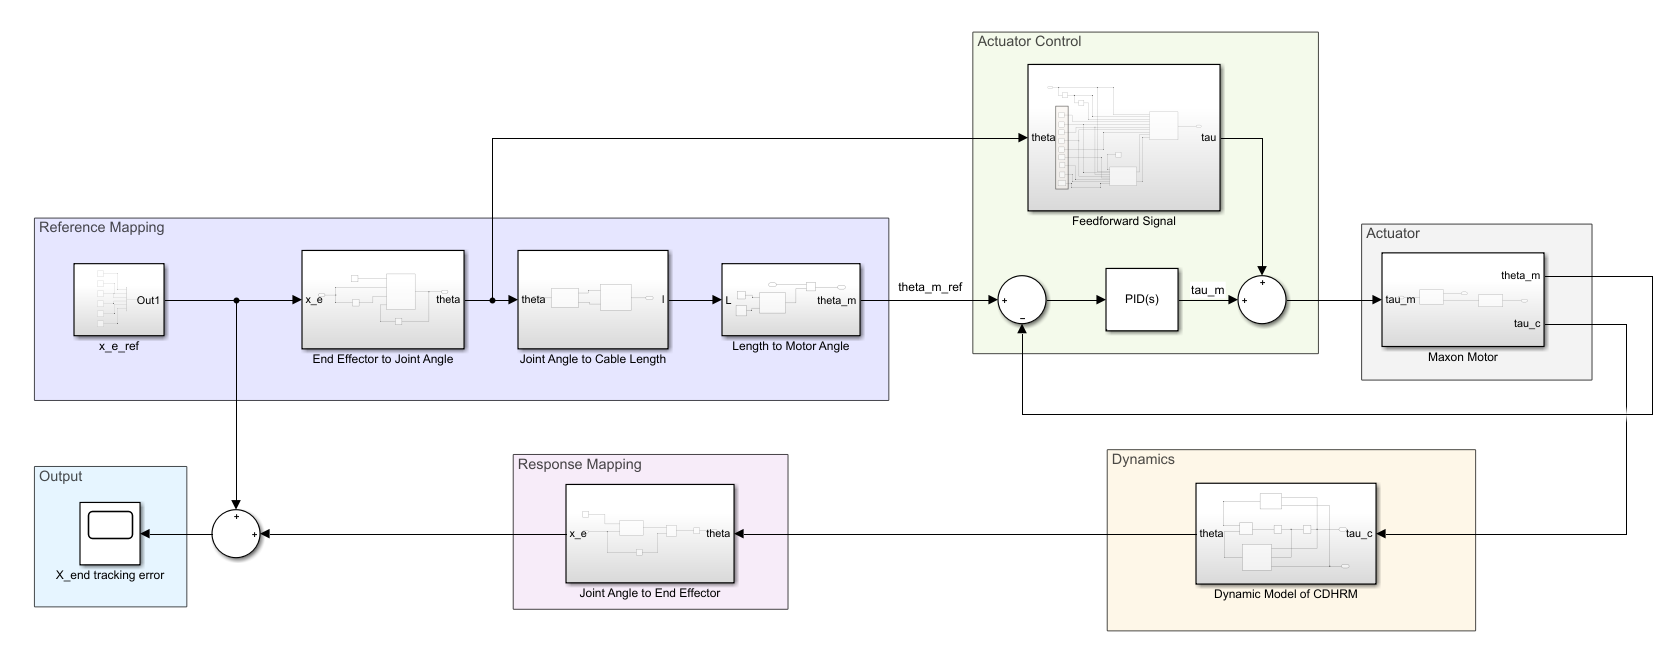
\includegraphics[width=\textwidth]{images/CDHRM_model.png}
	\end{figure}
	
	\section{Kinematic Model}
	\subsection{Cable Length to Motor Angle}
	\begin{figure}[H]
		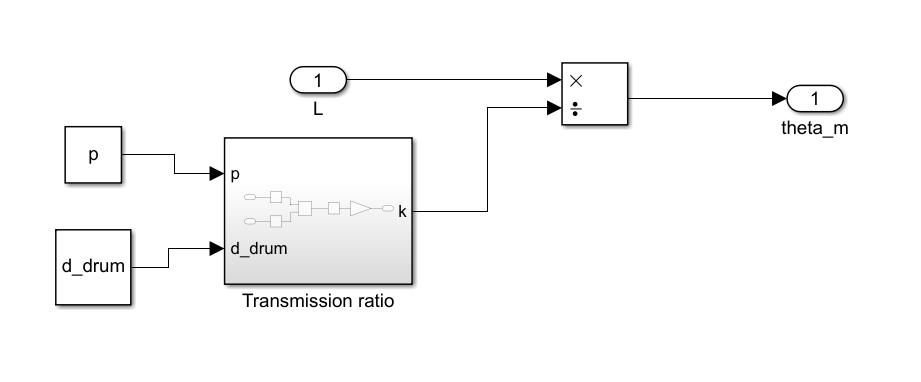
\includegraphics[width=\textwidth]{images/g1-inv.png}
	\end{figure}
	\subsection{Cable Length $\leftrightarrow$ Joint Angle}
	
	\subsubsection{Cable Length to Joint Angle}
	\begin{figure}[H]
		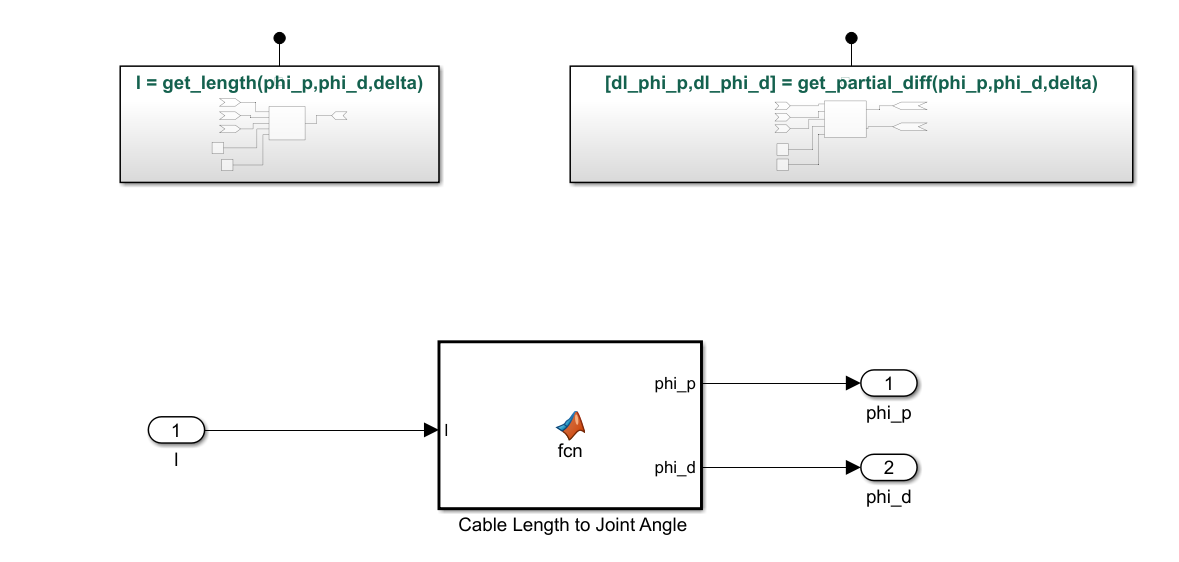
\includegraphics[width=\textwidth]{images/g2.png}
	\end{figure}
	\subsubsection{Joint Angle to Cable Length}
	\begin{figure}[H]
		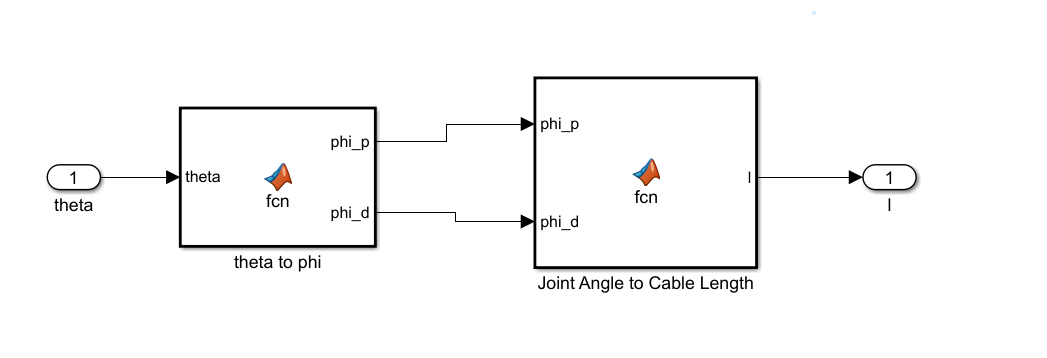
\includegraphics[width=\textwidth]{images/g2-inv.png}
	\end{figure}
	
	\subsection{End-effector position $\leftrightarrow$ Joint Angle}

	\subsubsection{End-effector position to Joint Angle}
	\begin{figure}[H]
		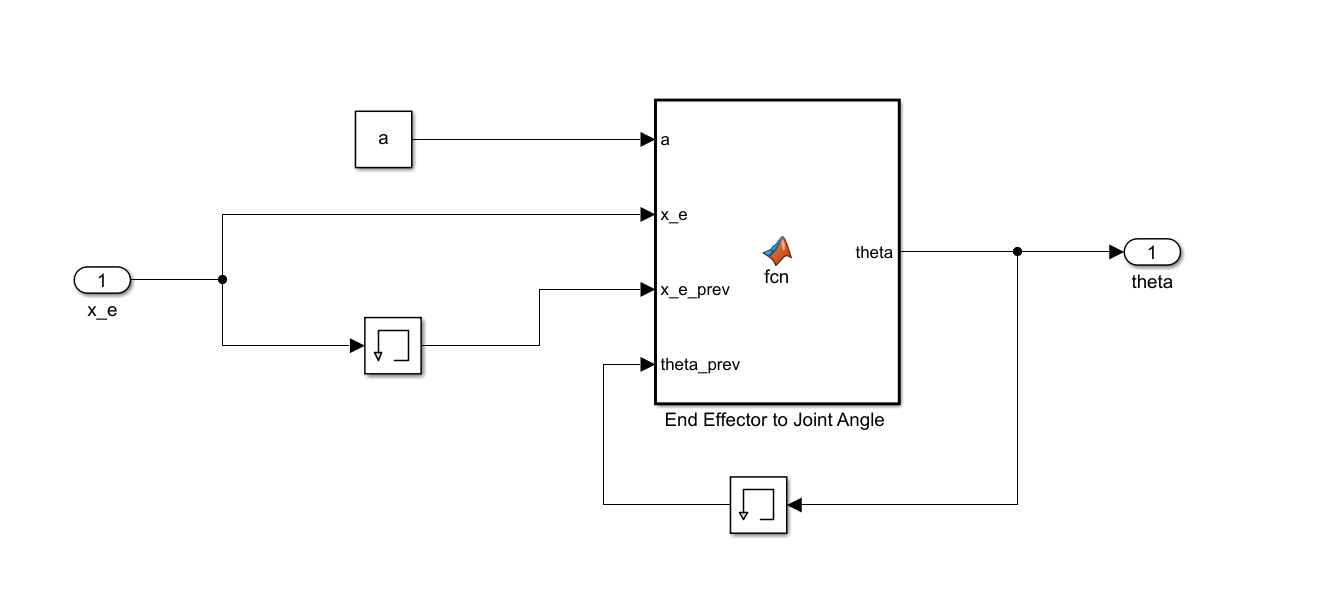
\includegraphics[width=\textwidth]{images/g3-inv.png}
	\end{figure}
	\subsubsection{Joint Angle to End-effector position}
	\begin{figure}[H]
		\includegraphics[width=\textwidth]{images/g3.png}
	\end{figure}
	
	\section{Dynamic Model (Forward Dynamics)}
	\begin{figure}[H]
		\includegraphics[width=\textwidth]{images/Dynamic-Model_BD.png}
	\end{figure}

	\section{Feedforward Block (Inward Dynamics)}
	\label{appendix d:4}
	\begin{figure}[H]
		\includegraphics[width=\textwidth]{images/Feedforward-block-in-model.png}
	\end{figure}
	
	\section{Actuator Block}
	\subsection{Inside the Actuator Block}
	\begin{figure}[H]
		\includegraphics[width=\textwidth]{images/Actuator-block.png}
	\end{figure}
	\subsection{Modelling the Maxon Motor}
	\begin{figure}[H]
		\includegraphics[width=\textwidth]{images/maxon-motor-model.png}
	\end{figure}
	\subsection{Converting Speed to Torque}
	\begin{figure}[H]
		\includegraphics[width=\textwidth]{images/speed-to-torque.png}
	\end{figure}
	\subsection{Tuning the Actuator}
	\begin{figure}[H]
		\includegraphics[width=\textwidth]{images/Motor-tuning.png}
	\end{figure}
	
	
	%%%%%%%%%%%%%%%%%
	
	\chapter{MATLAB Code}
	\label{appendix:c}
	
	This chapter of the appendix lists the code associated to the some of main blocks of the proposed control scheme that used MATLAB functions. All the code and Simulink models associated to the work undertaken as part of this project can be found in: \\ \url{https://github.com/Aru2612/BEng-Project-Control-of-CDHM}
	
	\section{Parameter Definition}
	
	This script defines the dynamic parameters and constants for the model. It is specified in the \texttt{InitFcn()}, and therefore is called automatically in the background every time the model is run.
	\lstinputlisting[language = Matlab]{code/parameters.m}
	
	\section{Kinematic Model: Cable Length - Joint Angles }
	\label{appendix:c-a}
	
	\subsection{Cable Length to Joint Angles}
	\lstinputlisting[language = Matlab]{code/cable_length_to_joint_angle.m}
	\subsubsection{Functions in this block}
	\lstinputlisting[language = Matlab]{code/functions_in_block.m}
	\subsubsection{$ \Phi $ to $ \Theta $ Conversion}
	\lstinputlisting[language = Matlab]{code/phi_to_theta.m}
	\subsubsection{$ \Theta $ to $ \Phi $ Conversion}
	\lstinputlisting[language = Matlab]{code/theta_to_phi.m}
	
	\subsection{Joint Angles to Cable Length}
	\lstinputlisting[language = Matlab]{code/joint_angle_to_cable_length.m}

	
	\section{Kinematic Model: Joint Angles - End-effector position Mapping}
	\label{appendix:c-b}
	
	\subsection{Joint Angles to End-effector position}
	\lstinputlisting[language = Matlab]{code/jacobian.m}
	
	\subsection{End-effector position to Joint Angles}
	\lstinputlisting[language = Matlab]{code/end_effector_to_joint_angle.m}
	
	\section{Dynamic Model}
	\subsection{Calculating Contact Forces}
	\lstinputlisting[language = Matlab]{code/contact_forces.m}
	\subsection{Newton-Euler Recursive Algorithm}
	\lstinputlisting[language = Matlab]{code/newton_euler.m}
	
\end{appendices}
%%%%%%%%%%%%%%%%%%%%%%%%%%%%%%%%%%%%%%

\bibliographystyle{IEEEtran}
\bibliography{references}

\end{document}